\clearpage

\section {Systematic effects in the prediction of the single $\mu$-like ring event energy spectrum}
\label{sec:systematics}

%....................................................................................................................
%....................................................................................................................

\subsection {Input systematic parameters}

\label{sec:systematics:inputs}

This analysis considers \NSyst{} systematic parameters which can be grouped into 3 categories:

\begin{enumerate}

\item 
{\bf Correlated flux and cross-section (BANFF) parameters} (37 parameters).\\

In this analysis, all the flux and cross-section systematic parameters are included in the ND280 data (BANFF) fit (in previous 
$\nu_{\mu}$-disappearance analyses, all the flux parameters but only a subset of the cross-section parameters were included).
There are 5 $\nu_{\mu}$, 11 $\bar{\nu}_{\mu}$, 2 $\nu_{e}$ and 7 $\bar{\nu}_{e}$ flux parameters as well as 12 cross-section parameters. 
Best-fit values of these parameters and a covariance matrix giving their correlated uncertainties are obtained by the BANFF group from a fit 
of the $\bar{\nu}_\mu$ and $\nu_\mu$ CC0$\pi$-like, CC1$\pi$-like and CC other-like ND280 samples as described in Ref~\cite{BANFF2015}. A list of the BANFF parameters, their best-fit values and their prefit and postfit errors is given in Tab.~\ref{tab:banff_uncertainties}. 
The best-fit values are used to reweight the templates as described in Sec.~\ref{sec:banff_weights}, and the postfit errors in the 
covariance matrix are used as prior uncertainties in this analysis. 

The effects of these correlated uncertainties are evaluated using the Cholesky method. The covariance matrix is ``Cholesky decomposed'' 
into the product of a lower triangular matrix (all elements above the diagonal are zero) and its transpose (in which all elements below the 
diagonal are zero). Random tweaks of each parameter are independently drawn from a Gaussian distribution with mean zero and standard deviation 1, 
and these random numbers are put into a vector. This vector is then multiplied by the lower triangular matrix to give a vector of tweaked 
uncertainties that have the correct correlations between them. The BANFF parameters are then varied by these tweaked uncertainties, with all 
parameters being varied simultaneously. This process may be repeated as many times as necessary. 

Some of the cross-section parameters have a complicated, often non-linear, dependence on true and reconstructed neutrino energy; the effects of 
uncertainties in these parameters are evaluated by reweighting the MC templates. Weights are calculated for tweaks from -3$\sigma$ to +3$\sigma$ 
in steps of 0.5$\sigma$, and interpolations are made between those weights using cubic splines (for MaQE only, weights are calculated from 
-7$\sigma$ to +3$\sigma$). Cubic splines are made for the following cross-section uncertainties:
\begin{itemize}
\item CCQE axial-mass scaling factor (MaQE)
\item Fermi momentum for $^{16}$O
\item Binding energy for $^{16}$O
\item Nucleon to $\Delta$ transition axial form factor (C$^{A}_{5}$) 
\item Resonance-production axial-mass scaling factor (MaRes)
\item Scale of isospin 1/2 nonresonant background
\item CC other shape
\end{itemize}
The splines are made in bins of true and reconstructed energy, and the binning is given in Ref.\ \cite{splineinfo}.

The effects of the flux and cross-section normalization uncertainties are also evaluated by reweighting the MC templates, but no splines are made for them
since the weight is identical to the tweak for these uncertainties (each flux parameter is a normalization for a limited range of true energy). 

The BANFF parameters are applied to the MC templates as specified in Tab.~\ref{tab:apply_syst_to_template}.

{
\renewcommand{\arraystretch}{1.2}
\begin{table}
\centering
\begin{tabular}{| c | c | c | c |}
\hline
           Parameter & Description & Best fit & 1$\sigma$ pre/postfit \\
           & & & fractional error \\
\hline
            0 &  $\nu_{\mu}$ flux normalisation, E = 0.0 - 0.7 GeV               & 1.142   & 0.094 / 0.071 \\ 
            1 &  $\nu_{\mu}$ flux normalisation, E = 0.7 - 1.0 GeV               & 1.091   & 0.079 / 0.053 \\ 
            2 &  $\nu_{\mu}$ flux normalisation, E = 1.0 - 1.5 GeV               & 1.079   & 0.077 / 0.052 \\ 
            3 &  $\nu_{\mu}$ flux normalisation, E = 1.5 - 2.5 GeV               & 1.074   & 0.081 / 0.060 \\ 
            4 &  $\nu_{\mu}$ flux normalisation, E = 2.5 - 30.0 GeV              & 1.050   & 0.080 / 0.053 \\ 
            5 &  $\bar{\nu}_{\mu}$ flux normalisation, E = 0.0 - 0.4 GeV         & 1.204   & 0.104 / 0.069 \\ 
            6 &  $\bar{\nu}_{\mu}$ flux normalisation, E = 0.4 - 0.5 GeV         & 1.210   & 0.102 / 0.058 \\ 
            7 &  $\bar{\nu}_{\mu}$ flux normalisation, E = 0.5 - 0.6 GeV         & 1.180   & 0.096 / 0.051 \\ 
            8 &  $\bar{\nu}_{\mu}$ flux normalisation, E = 0.6 - 0.7 GeV         & 1.128   & 0.085 / 0.041 \\ 
            9 &  $\bar{\nu}_{\mu}$ flux normalisation, E = 0.7 - 1.0 GeV         & 1.123   & 0.125 / 0.077 \\ 
           10 &  $\bar{\nu}_{\mu}$ flux normalisation, E = 1.0 - 1.5 GeV         & 1.118   & 0.105 / 0.068 \\ 
           11 &  $\bar{\nu}_{\mu}$ flux normalisation, E = 1.5 - 2.5 GeV         & 1.121   & 0.080 / 0.053 \\ 
           12 &  $\bar{\nu}_{\mu}$ flux normalisation, E = 2.5 - 3.5 GeV         & 1.121   & 0.074 / 0.049 \\ 
           13 &  $\bar{\nu}_{\mu}$ flux normalisation, E = 3.5 - 5.0 GeV         & 1.122   & 0.094 / 0.067 \\ 
           14 &  $\bar{\nu}_{\mu}$ flux normalisation, E = 5.0 - 7.0 GeV         & 1.112   & 0.093 / 0.064 \\ 
           15 &  $\bar{\nu}_{\mu}$ flux normalisation, E = 7.0 - 30.0 GeV        & 1.093   & 0.130 / 0.108 \\ 
           16 &  $\nu_{e}$ flux normalisation, E = 0.0 - 2.5 GeV                 & 1.109   & 0.069 / 0.047 \\ 
           17 &  $\nu_{e}$ flux normalisation, E = 2.5 - 30.0 GeV                & 1.090   & 0.085 / 0.067 \\ 
           18 &  $\bar{\nu}_{e}$ flux normalisation, E = 0.0 - 0.5 GeV           & 1.193   & 0.095 / 0.054 \\ 
           19 &  $\bar{\nu}_{e}$ flux normalisation, E = 0.5 - 0.7 GeV           & 1.184   & 0.091 / 0.047 \\ 
           20 &  $\bar{\nu}_{e}$ flux normalisation, E = 0.7 - 0.8 GeV           & 1.167   & 0.091 / 0.049 \\ 
           21 &  $\bar{\nu}_{e}$ flux normalisation, E = 0.8 - 1.5 GeV           & 1.141   & 0.084 / 0.044 \\ 
           22 &  $\bar{\nu}_{e}$ flux normalisation, E = 1.5 - 2.5 GeV           & 1.120   & 0.080 / 0.054 \\ 
           23 &  $\bar{\nu}_{e}$ flux normalisation, E = 2.5 - 4.0 GeV           & 1.123   & 0.089 / 0.068 \\ 
           24 &  $\bar{\nu}_{e}$ flux normalisation, E = 4.0 - 30.0 GeV          & 1.180   & 0.156 / 0.144 \\ 
           25 &  Meson exchange current normalisation for $^{16}$O               & 1.031   & 1.041 / 1.015 \\ 
           26 &  C$^{A}_{5}$ nucleon to $\Delta$ transition axial form factor    & 0.854   & 0.119 / 0.073 \\ 
           27 &  Scale of isospin 1/2 nonresonant background                     & 1.143   & 0.154 / 0.146 \\ 
           28 &  CCQE axial-mass scaling factor                                  & 0.948   & 0.058 / 0.028 \\ 
           29 &  Resonance-production axial-mass scaling factor                  & 0.762   & 0.158 / 0.055 \\ 
           30 &  Fermi momentum for $^{16}$O                                     & 0.997   & 0.055 / 0.054 \\ 
           31 &  CC other shape                                                  & 0.023   & 0.400 / 0.193 \\ 
           32 &  Binding energy for $^{16}$O                                     & 1.002   & 0.333 / 0.326 \\ 
           33 &  CC coherent for $^{16}$O normalisation                          & 1.076   & 1.000 / 0.972 \\ 
           34 &  NC coherent normalisation                                       & 0.980   & 0.300 / 0.299 \\ 
           35 &  NC other normalisation                                          & 1.413   & 0.300 / 0.186 \\ 
           36 &  CC $\nu_{e}$ normalisation                                      & 1.001   & 0.020 / 0.020 \\ 
\hline
\end{tabular}
\caption{
 Summary of flux and correlated cross-section (BANFF) systematics included in the {\em VALOR} Run 5+6 
 $\bar{\nu}_{\mu}$-disappearance analysis.
 A description of how the BANFF fit constrained these systematics can be found in Ref.~\cite{BANFF2015}.
}
\label{tab:banff_uncertainties}
\end{table}
}

\clearpage


\item
{\bf SuperK efficiencies \& effects of intranuclear and secondary re-interactions} (12 parameters).\\

There are uncertainties in the efficiencies of the fiducial volume and reduction chain,
and the OD, ring-counting, PID, momentum and decay-electron cuts.
These uncertainties have been evaluated by comparing 1412 days of SK-IV atmospheric data
with atmospheric neutrino Monte Carlo.
Ring counting errors are evaluated using $\nu_\mu$ CCQE, $\nu_\mu$ CCnQE, NC, and $\nu_e$ CC-enriched control samples.
The NC PID error is evaluated using a NC-enriched control sample, which
does not use PID information.
Each Monte Carlo control sample is fitted to the data using the efficiency as a fit parameter, and the uncertainties in the
efficiencies are estimated by adding the covariance matrix containing the differences between the best-fit and nominal efficiencies to
the covariance matrix containing the statistical errors in the fitted efficiencies \cite{SuperkErrors2013}.

Intranuclear final-state interactions (FSI) have significant effects in the T2K energy range and
result in event topologies, for scattering from nuclear targets, which are drastically different from
those created in neutrino scattering from free nucleons.
Uncertainties due to FSI were estimated by simultaneously varying the NEUT parameters that scale the interaction probabilities for quasi-elastic
scattering, absorption, charge exchange and pion production using the method described in Sec.\ 2 in \cite{NIWGErr}. The NIWG group produced 16
parameter sets that span the 1$\sigma$ surface in the parameter space; this was done by varying the NEUT parameters when running the pion scattering
simulations, and comparing the results with external pion-carbon scattering data. These 16 parameter sets are shown in Tab.\ 2 in \cite{NIWGErr}.
Uncertainties due to secondary pion interactions (SI) were also evaluated. The NIWG group adapted the NEUT nuclear cascade model to simulate SI in the
SuperK detector simulation (SKDETSIM) and to allow variations in the interaction probabilities. Details of this are given in \cite{SI}.
Since the same model is used for FSI and SI, it is possible to evaluate the uncertainties in both FSI and SI simultaneously. This was done by
reweighting a single $e$-like ring selected SK MC with the 16 FSI parameter sets using T2KReweight. The reweighting method for FSI is described
in Sec.\ 8 in \cite{NEUTnuclear}. Variations in the SI interaction probabilities were included for each FSI parameter set.  Subsequently a covariance
matrix was calculated using equation 1 in \cite{NIWGErr}; the quantity p in that equation is the average event weight for a FSI parameter set, and
the sum is over the parameter sets.




{
\renewcommand{\arraystretch}{1.5}



\begin{table}
\centering
\begin{tabular}{| c | c | c |}
\hline
 Parameter               &  Definition  &  1$\sigma$ error   \\
\hline
%   1       &  $\nu_\mu$ and $\bar{\nu}_{\mu}$ CCQE, $E_{reco}<$ 0.4 GeV                    &  0.018    \\
%   2       &  $\nu_\mu$ and $\bar{\nu}_{\mu}$ CCQE, 0.4 GeV $\leq E_{reco} \leq$ 1.1 GeV   &  0.016    \\
%   3       &  $\nu_\mu$ and $\bar{\nu}_{\mu}$ CCQE, $E_{reco}>$ 1.1 GeV                    &  0.016    \\
%   4       &  $\nu_\mu$ and $\bar{\nu}_{\mu}$ CCnonQE                                      &  0.093    \\
%   5       &  $\nu_e$   and $\bar{\nu}_{e}$ CC                                             &  1.006    \\
%   6       &  All NC                                                                       &  0.598    \\

1           & oscillated $\nu_e$ CC, $E_{reco}<$ 0.35 GeV              & 0.059      \\ 
2           & oscillated $\nu_e$ CC, 0.35 $<E_{reco}<$ 0.80 GeV                & 0.027      \\ 
3           & oscillated $\nu_e$ CC, 0.80 $<E_{reco}<$ 1.25 GeV                & 0.056      \\ 
4           & $\nu_\mu$ and $\bar{\nu}_{\mu}$ CC, $E_{reco}<$ 0.35 GeV                & 1.241      \\ 
5           & $\nu_\mu$ and $\bar{\nu}_{\mu}$ CC, 0.35 $<E_{reco}<$ 0.80 GeV       & 1.129       \\ 
6           & $\nu_\mu$ and $\bar{\nu}_{\mu}$ CC, 0.80 $<E_{reco}<$ 1.25 GeV       & 0.917        \\ 
7           & $\nu_e$   and $\bar{\nu}_{e}$ CC, $E_{reco}<$ 0.35 GeV    		   & 0.044        \\ 
8           & $\nu_e$   and $\bar{\nu}_{e}$ CC, 0.35 $<E_{reco}<$ 0.80 GeV      	 & 0.032        \\ 
9           & $\nu_e$   and $\bar{\nu}_{e}$ CC, 0.80 $<E_{reco}<$ 1.25 GeV      	 & 0.068        \\ 
10         & all NC, $E_{reco}<$ 0.35 GeV      	 & 0.476        \\ 
11         & all NC, 0.35 $<E_{reco}<$ 0.80 GeV      	 & 0.301        \\ 
12         & all NC, 0.80 $<E_{reco}<$ 1.25 GeV      	 & 0.608        \\ 
\hline
\end{tabular}
\caption{
  Binning of SuperK selection efficiency and FSI+SI systematic parameters in covariance matrices
}
\label{tab:fsi_si_params}
\end{table}
}

We consider the SuperK detector efficiency and FSI+SI systematics together, and add their covariance matrices linearly. Each of
these covariance matrices has 12 correlated parameters, corresponding to different modes and reconstructed energy bins, as shown in
Tab.~\ref{tab:fsi_si_params}. The effects of these uncertainties are also evaluated using the Cholesky method. \\

\item
{\bf SuperK energy scale} (1 parameter).\\

The systematic parameter $f_{E; r}^{SK}$ is included to estimate the effects of uncertainty in the SuperK reconstructed energy scale.
This uncertainty is estimated to be 2.4\% \cite{SuperkEScale2013}; its effects are calculated by scaling the bin edges of
the MC templates and, assuming uniform distribution of events within the bins, calculating the number
of events gained from / lost to neighbouring bins.
The effect of the energy scale uncertainty is propagated to all MC templates as shown in Tab.~\ref{tab:apply_syst_to_template}. \\


\item 
{\bf Oscillation parameters and mass hierarchy} (7 parameters).\\

The 3-flavour oscillation probability is used. 
The mass hierarchy and the following oscillation parameters are randomly extracted from
the posterior distribution of the T2K+reactor joint Mach3 bayesian analysis ~\cite{Mach3JointFitRun14}.
A discrete prior is used for the mass hierarchy:  the probability for normal hierarchy (NH) and 
inverted hierarchy (IH) is respectively 0.684 and 0.326.
Different priors of the oscillation parameters are used for NH and IH.
$\sin^{2}\theta_{23}$ and $|\Delta m^{2}_{32}|$ for NH ($|\Delta m^{2}_{31}|$ for IH)
are randomly extracted from the 2D prior distribution shown in Fig.~\ref{fig:prior_mix23_dmsq},
taking into account the existing correlations.
$\sin^{2}\theta_{13}$ and $\delta_{CP}$ are extracted from the 2D prior distribution shown
in Fig.~\ref{fig:prior_mix13_dcp} taking into account the correlations.

\begin{figure}
\center
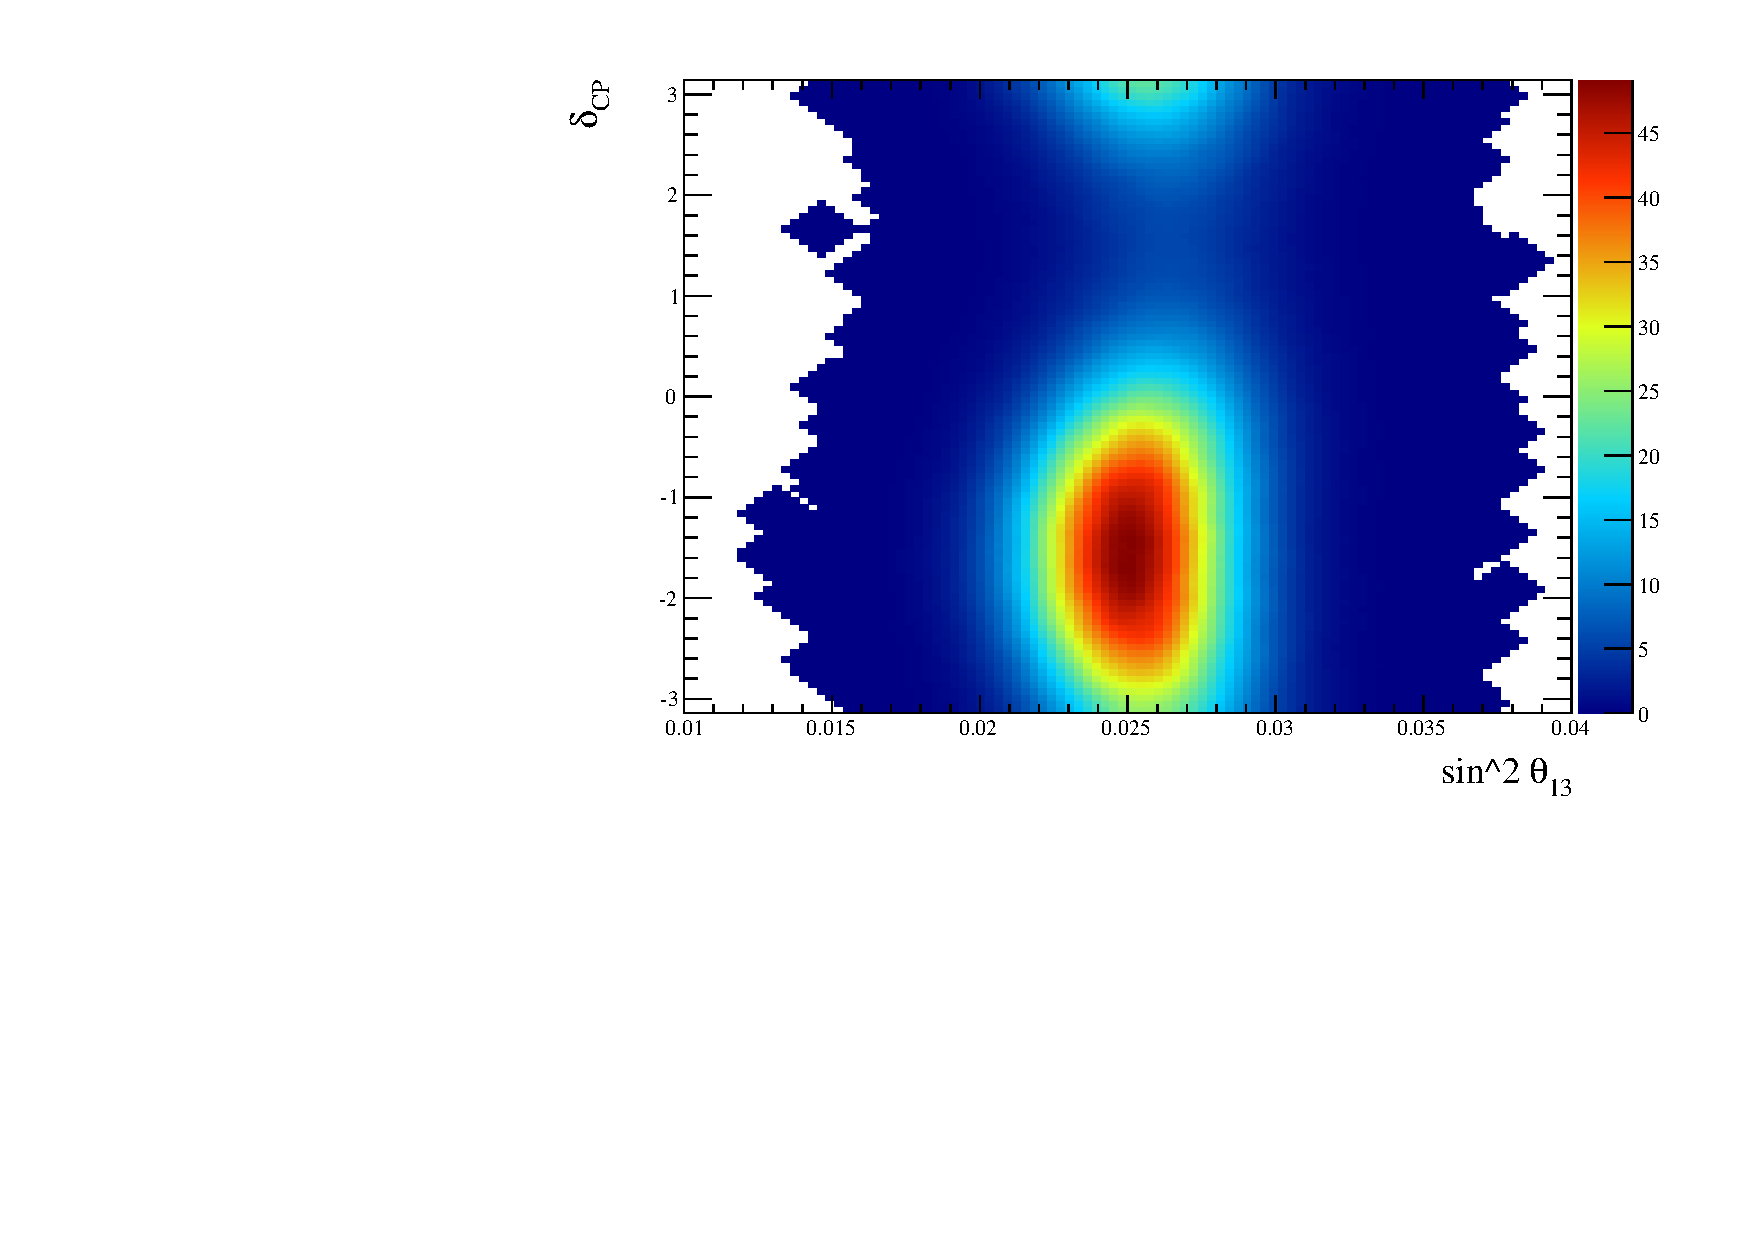
\includegraphics[width=0.48\linewidth]{./nuebar_plots/osc_prior/mix13_dcp_nh.pdf}
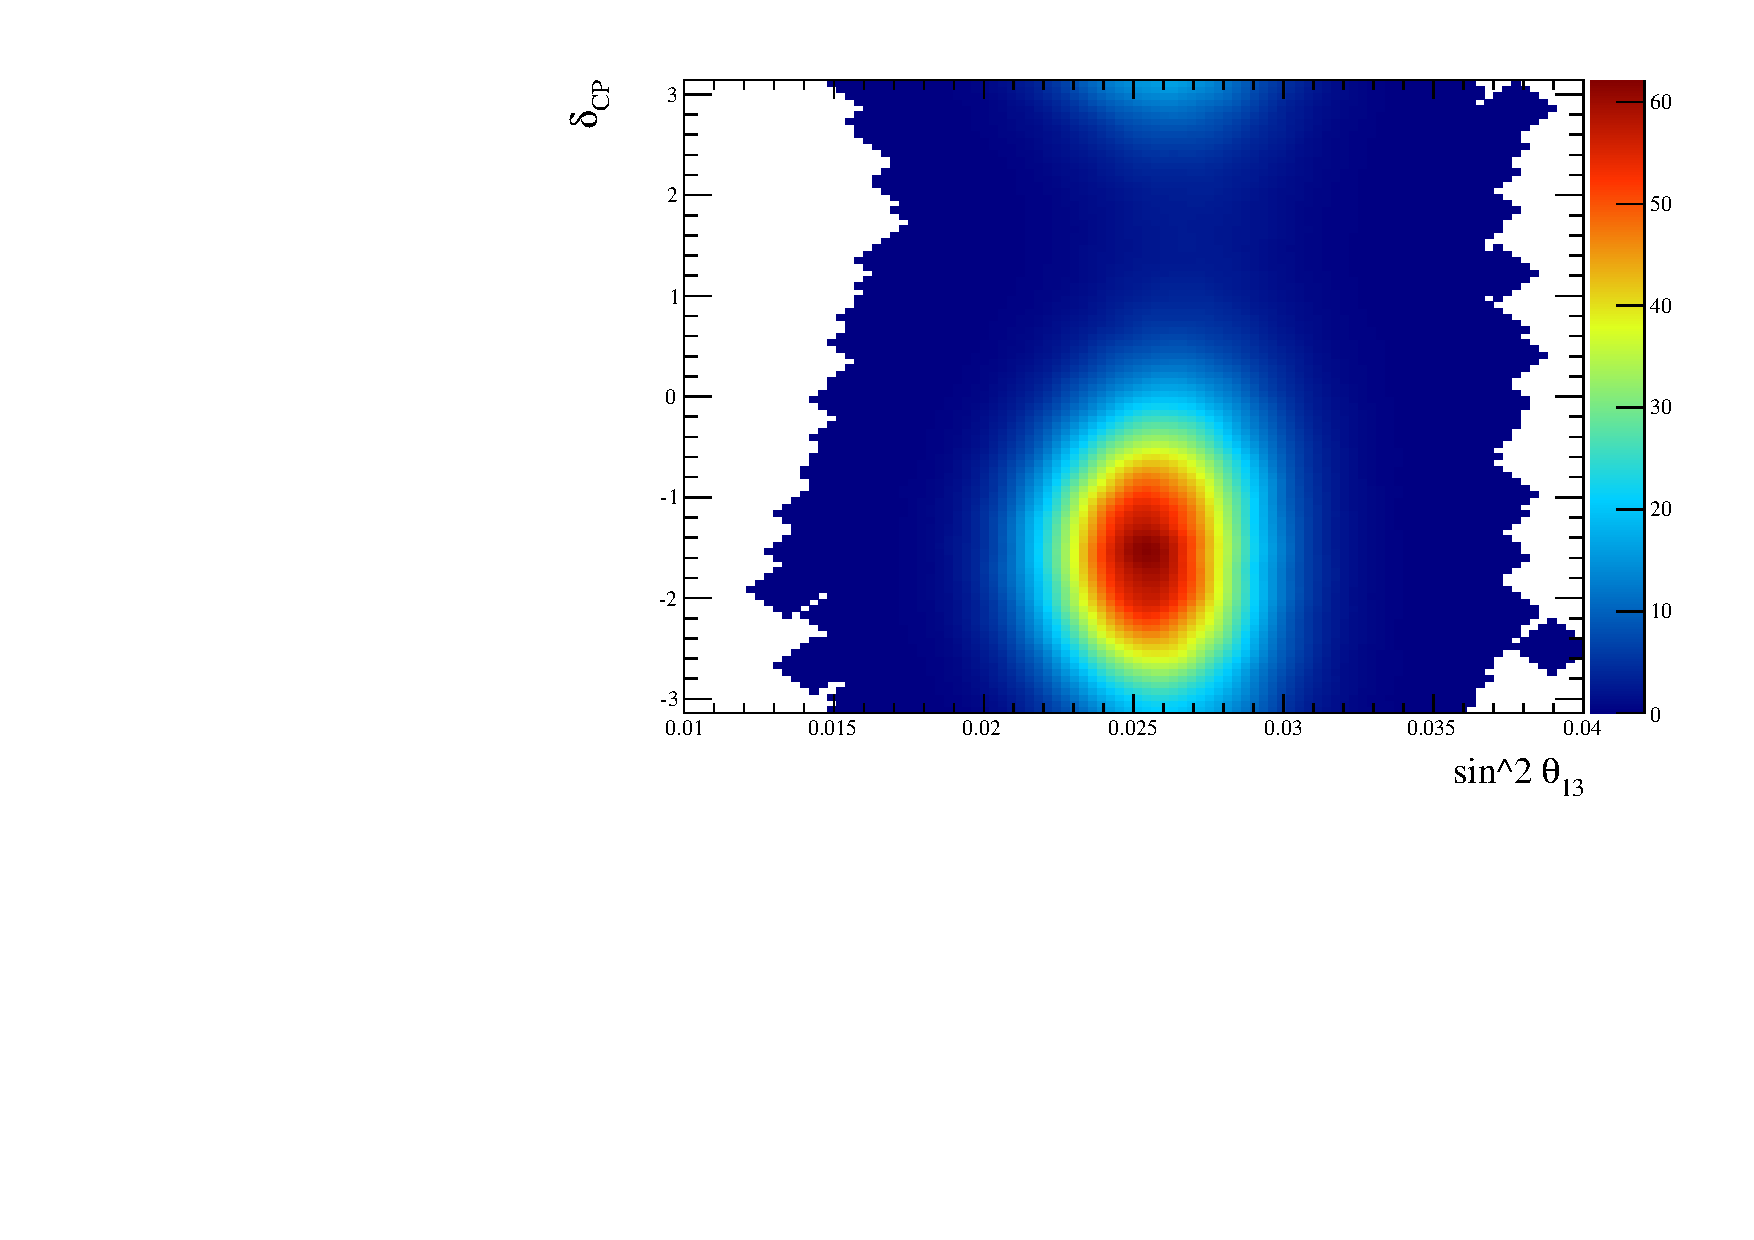
\includegraphics[width=0.48\linewidth]{./nuebar_plots/osc_prior/mix13_dcp_ih.pdf}
\caption {
Prior distributions used to randomly extract $\sin^{2}\theta_{13}$ and $\delta_{CP}$
for NH (left) and IH (right).
The correlations between the parameters are taken into account. 
The distributions are from the T2K+reactor joint Mach3 bayesian analysis ~\cite{Mach3JointFitRun14}.
}
\label{fig:prior_mix13_dcp}
\end{figure}

\begin{figure}
\center
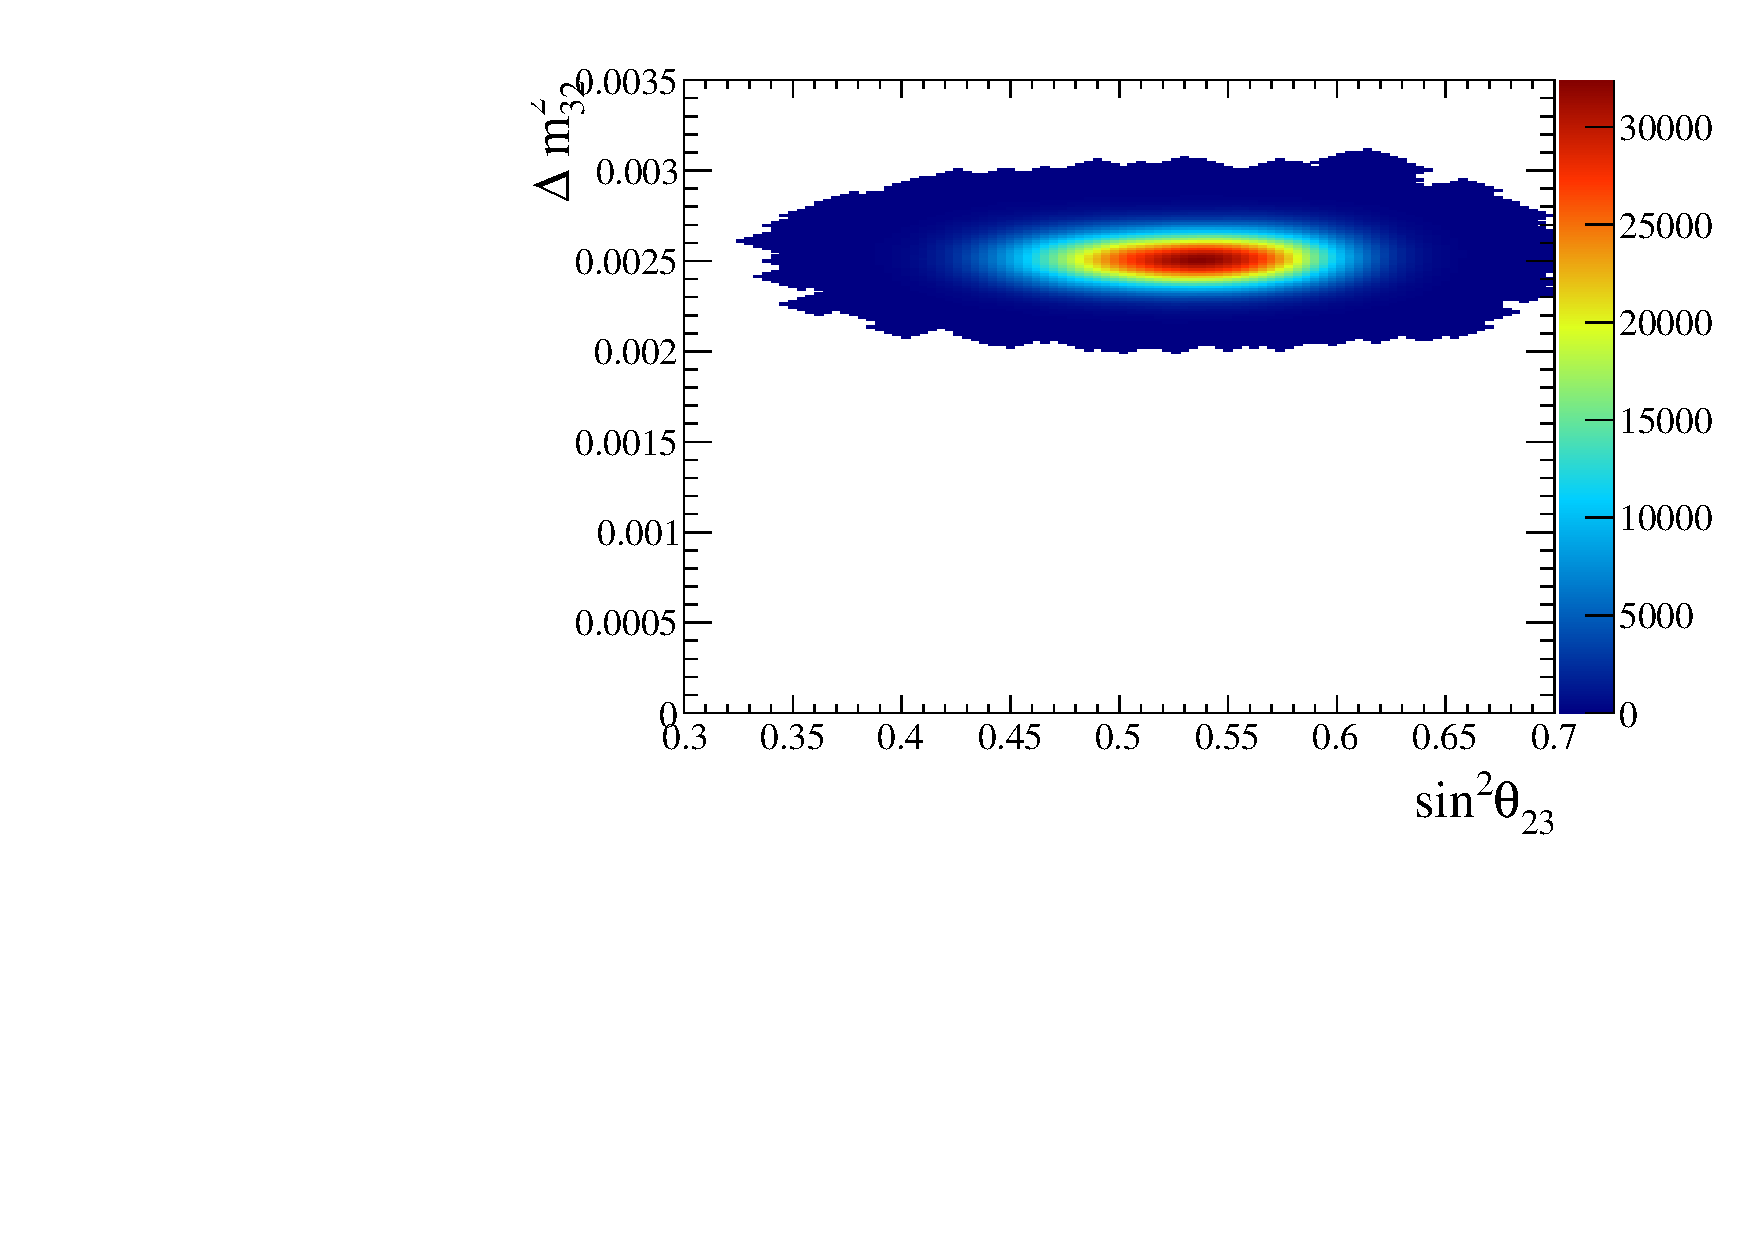
\includegraphics[width=0.48\linewidth]{./nuebar_plots/osc_prior/mix23_dmsq_nh.pdf}
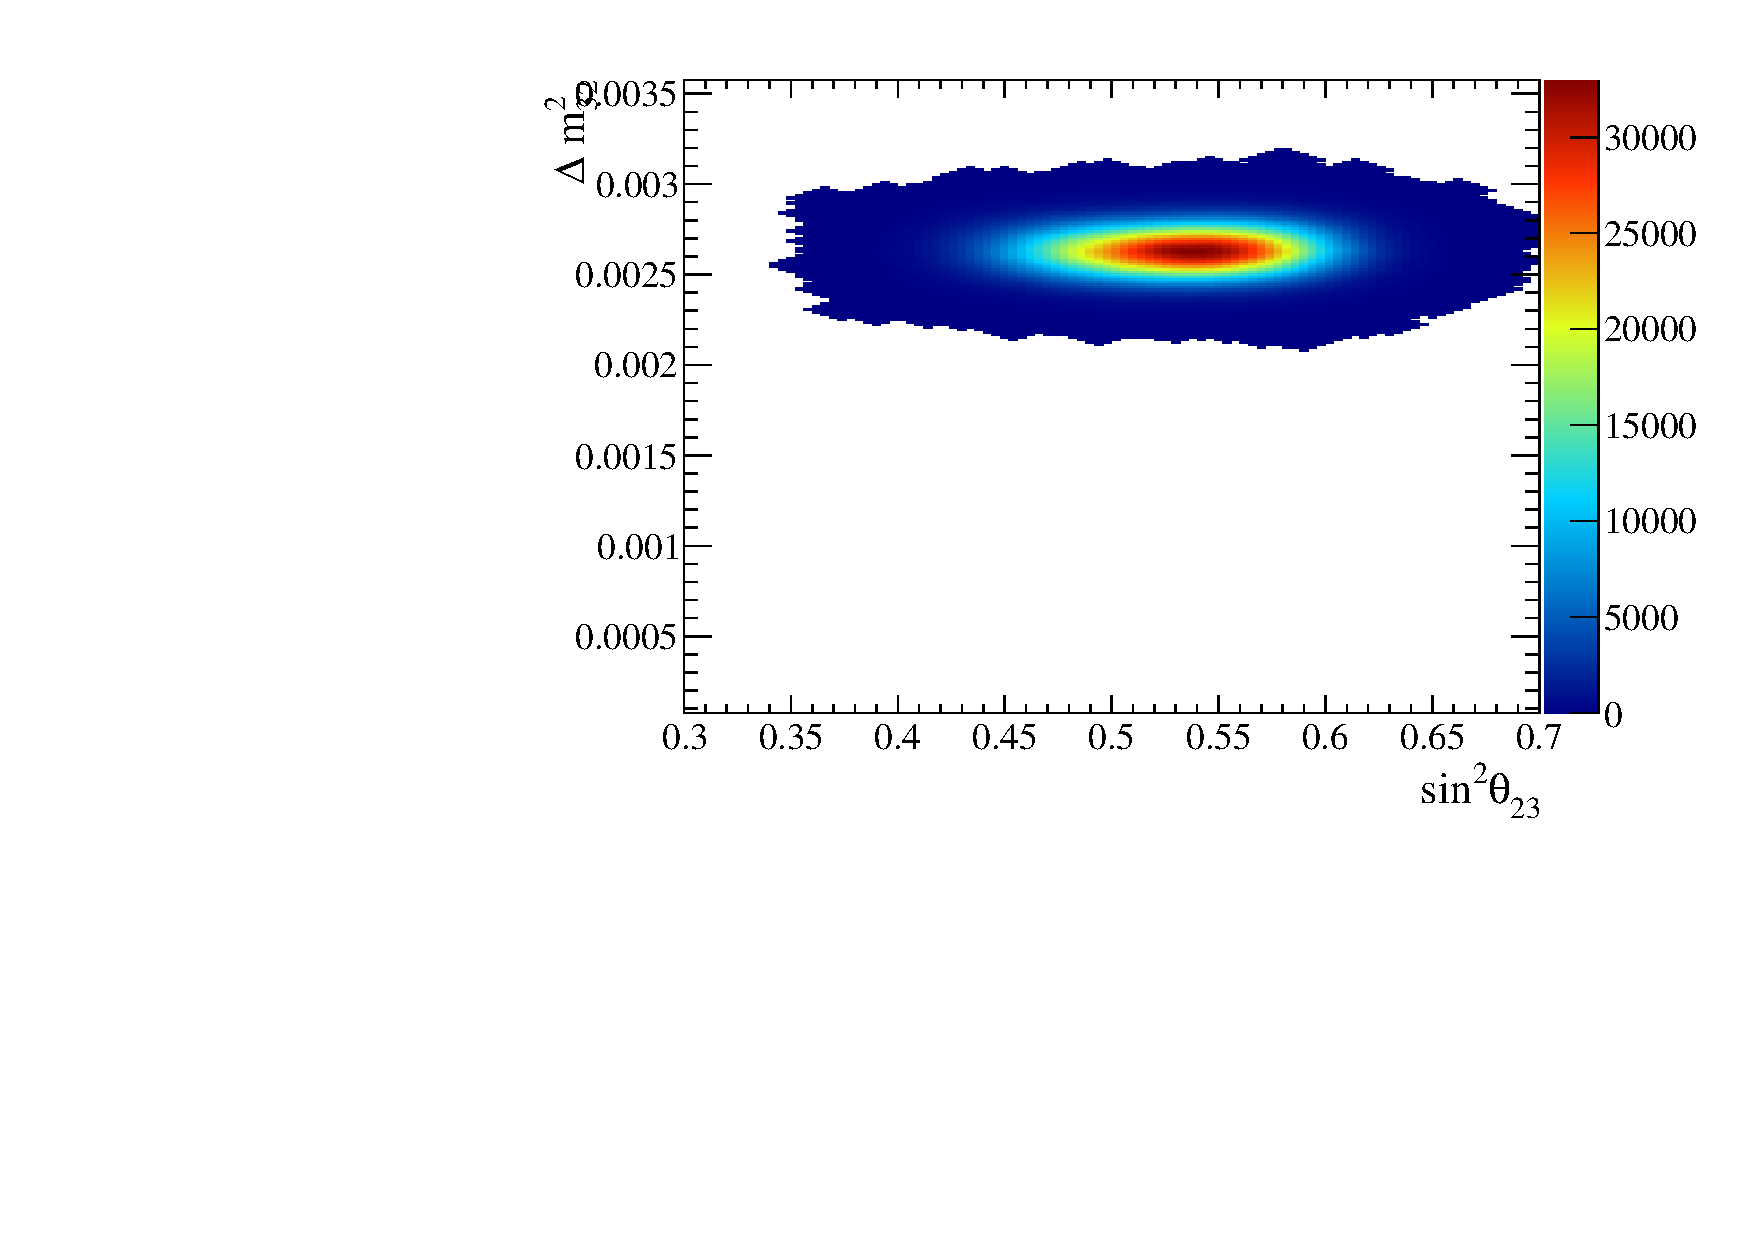
\includegraphics[width=0.48\linewidth]{./nuebar_plots/osc_prior/mix23_dmsq_ih.pdf}
\caption {
Prior distributions used to randomly extract $\sin^{2}\theta_{23}$ and $|\Delta m^{2}_{32}|$ for NH (left),
$\sin^{2}\theta_{23}$ and $|\Delta m^{2}_{31}|$ for IH (right).
The correlations between the parameters are taken into account. 
The distributions are from the T2K+reactor joint Mach3 bayesian analysis ~\cite{Mach3JointFitRun14}.
}
\label{fig:prior_mix23_dmsq}
\end{figure}

The treatment of the oscillation parameters in the analysis as well as the nominal values
are shown in Tab.~\ref{tab:osc_params_fixed_values_reactor}.

\begin{table}
\centering
 \begin{tabular}{| c | c | c |}
% \hline
% Parameter(s)                                               			&     Treatment              &           Nominal value (NH)           & Nominal value (IH)      \\
%\hline
%$\sin^{2}\theta_{23}$                                       			&     marginalized         &                \MixingTwoThreeNH       &    \MixingTwoThreeIH  \\
%$\sin^{2}\theta_{13}$  							&     marginalized         &                \MixingOneThreeNH	&      \MixingOneThreeIH	 \\
%$\sin^{2}\theta_{12}$  							&     fixed               	    &             \MixingOneTwoIH             &    \MixingOneTwoIH	 \\
%$|\Delta m^{2}_{32}|$ (NH) / $|\Delta m^{2}_{31}|$ (IH)      &     marginalized          &               \DmsqNH			&      \DmsqIH                        \\
%$\Delta m^{2}_{21}$      							&     fixed                       &             \dmsqIH                          & 	\dmsqIH		\\
%$\delta_{CP}$                                               			&     marginalized           &              \DeltaCPNH			&     \DeltaCPIH              \\
%Mass Hierarchy									&     marginalized	    &           Normal Hierarchy
 \hline
 Parameter(s)                                               			&     Treatment              &           Nominal value 		    \\
\hline
$\sin^{2}\theta_{23}$                                       			&     marginalized         &                \MixingTwoThreeNH        \\
$\sin^{2}\theta_{13}$  							&     marginalized         &                \MixingOneThreeNH	 \\
$\sin^{2}\theta_{12}$  							&     fixed               	    &             \MixingOneTwoIH              \\
$|\Delta m^{2}_{32}|$ (NH) / $|\Delta m^{2}_{31}|$ (IH)      &     marginalized          &               \DmsqNH		          \\
$\Delta m^{2}_{21}$      							&     fixed                       &             \dmsqIH                         	\\
$\delta_{CP}$                                               			&     marginalized           &              \DeltaCPNH		      \\
Mass Hierarchy									&     marginalized	    &            	NH         \\  
\hline
\end{tabular}
\caption{
Treatment of the oscillation parameters in the p-value computation as well as used values for fixed parameters.
The values of the fixed oscillation parameters correspond to the most probable parameters of the bayesian analysis
described in \cite{T2KLongPaper,Mach3JointFitRun14}.
The mass hierarchy is marginalized as well.
}
\label{tab:osc_params_fixed_values_reactor}
\end{table}


The effect of the oscillation parameters on the total number of superK events is shown in Tab.~\ref{tab:osc_params_systeffect}.
How the effect of each single oscillation parameter is mixed with the others is not trivial.
Indeed priors with correlations for $\sin^{2}\theta_{23}$ and $|\Delta m^{2}_{32}|$ (NH) / $|\Delta m^{2}_{31}|$ (IH)
and for $\sin^{2}\theta_{13}$ and $\delta_{CP}$  are used.
Furthermore, since a 3-flavour oscillation probability is used, when the oscillation parameters are 
randomly extracted together additional correlations are introduced as well.

\begin{table}
\centering
 \begin{tabular}{| c | c |}
 \hline
 Parameter(s)                                               								&     1$\sigma$ effect (Std. Dev. / Mean)                    \\
\hline
$\sin^{2}\theta_{12}$  												&      -              	    	\\
$\Delta m^{2}_{21}$      												&      -                        	\\
$\sin^{2}\theta_{23}$                                       								&      0.082            	\\
$|\Delta m^{2}_{32}|$ (NH) / $|\Delta m^{2}_{31}|$ (IH)     						 &      0.044              	\\
$\sin^{2}\theta_{13}$  												&      0.086         	\\
$\delta_{CP}$                                               								&      0.085              	\\
\hline
$\sin^{2}\theta_{13}$  \& $\delta_{CP}$                              						 &      0.117              	\\
$\sin^{2}\theta_{23}$  \& $|\Delta m^{2}_{32}|$ (NH) / $|\Delta m^{2}_{31}|$ (IH)    	&     0.082             	\\
\hline
all																&     0.135 		\\
\hline
\end{tabular}
\caption{
1$\sigma$ effect on the total number of superK events as the standard deviation divided by the mean of the distribution
given by the oscillation parameters.
$\sin^{2}\theta_{12}$ and $\Delta m^{2}_{21}$ are kept fixed.
The mass hierarchy is always randomly extracted. The priors described above are used and
correlations between parameters are taken into account when existing.
\NumToys toys are performed setting $\beta=1$.
}
\label{tab:osc_params_systeffect}
\end{table}




\end{enumerate}

%\afterpage{%\documentclass[10pt]{article}
%\usepackage[utf8]{inputenc}
%\usepackage{amsmath}
%\usepackage{amsfonts}
%\usepackage{amssymb}
%\usepackage{fullpage}
%\usepackage{rotate}  
%\usepackage{rotating}
%\usepackage[paperwidth=300mm,paperheight=450mm]{geometry}

%\newcommand{\ck}{$\checkmark$}
%\begin{document}

{
\setlength{\tabcolsep}{3pt}
\renewcommand{\arraystretch}{1.8}
\begin{landscape}
\begin{footnotesize}
\begin{longtable} { | c ||c | c | c | c | c | c | c | c | c | c | c | c | c | c | c | c | c | c | c | c | c | c | c | c | c | c | c | c | c | c | c | c | c | c | c | c | c | c | c | c | c | c | c | c | c | c |  | }
\hline
 & \begin{sideways} $\nu_\mu$ CCQE \end{sideways} 
 & \begin{sideways} $\nu_\mu$ CC 1$\pi$ \end{sideways} 
 & \begin{sideways} $\nu_\mu$ CC coherent \end{sideways} 
 & \begin{sideways} $\nu_\mu$ CC MEC \end{sideways} 
 & \begin{sideways} $\nu_\mu$ CC other \end{sideways} 
 & \begin{sideways} $\nu_\mu$/$\nu_\tau$ NC 1$\pi^{+/-}$ \end{sideways} 
 & \begin{sideways} $\nu_\mu$/$\nu_\tau$ NC 1$\pi^0$ \end{sideways} 
 & \begin{sideways} $\nu_\mu$/$\nu_\tau$ NC coherent \end{sideways} 
 & \begin{sideways} $\nu_\mu$/$\nu_\tau$ NC other \end{sideways} 
 & \begin{sideways} $\bar{\nu}_\mu$ CCQE \end{sideways} 
 & \begin{sideways} $\bar{\nu}_\mu$ CC 1$\pi$ \end{sideways} 
 & \begin{sideways} $\bar{\nu}_\mu$ CC coherent \end{sideways} 
 & \begin{sideways} $\bar{\nu}_\mu$ CC MEC \end{sideways} 
 & \begin{sideways} $\bar{\nu}_\mu$ CC other \end{sideways} 
 & \begin{sideways} $\bar{\nu}_\mu$/$\bar{\nu}_\tau$ NC 1$\pi^{+/-}$ \end{sideways} 
 & \begin{sideways} $\bar{\nu}_\mu$/$\bar{\nu}_\tau$ NC 1$\pi^0$ \end{sideways} 
 & \begin{sideways} $\bar{\nu}_\mu$/$\bar{\nu}_\tau$ NC coherent \end{sideways} 
 & \begin{sideways} $\bar{\nu}_\mu$/$\bar{\nu}_\tau$ NC other \end{sideways} 
 & \begin{sideways} $\nu_e$ CCQE \end{sideways} 
 & \begin{sideways} $\nu_e$ CC 1$\pi$ \end{sideways} 
 & \begin{sideways} $\nu_e$ CC coherent \end{sideways} 
 & \begin{sideways} $\nu_e$ CC MEC \end{sideways} 
 & \begin{sideways} $\nu_e$ CC other \end{sideways} 
 & \begin{sideways} $\nu_e$ NC 1$\pi^{+/-}$ \end{sideways} 
 & \begin{sideways} $\nu_e$ NC 1$\pi^0$ \end{sideways} 
 & \begin{sideways} $\nu_e$ NC coherent \end{sideways} 
 & \begin{sideways} $\nu_e$ NC other \end{sideways} 
 & \begin{sideways} Osc. $\nu_e$ CCQE \end{sideways} 
 & \begin{sideways} Osc. $\nu_e$ CC 1$\pi$ \end{sideways} 
 & \begin{sideways} Osc. $\nu_e$ CC coherent \end{sideways} 
 & \begin{sideways} Osc. $\nu_e$ CC MEC \end{sideways} 
 & \begin{sideways} Osc. $\nu_e$ CC other \end{sideways} 
 & \begin{sideways} $\bar{\nu}_e$ CCQE \end{sideways} 
 & \begin{sideways} $\bar{\nu}_e$ CC 1$\pi$ \end{sideways} 
 & \begin{sideways} $\bar{\nu}_e$ CC coherent \end{sideways} 
 & \begin{sideways} $\bar{\nu}_e$ CC MEC \end{sideways} 
 & \begin{sideways} $\bar{\nu}_e$ CC other \end{sideways} 
 & \begin{sideways} $\bar{\nu}_e$ NC 1$\pi^{+/-}$ \end{sideways} 
 & \begin{sideways} $\bar{\nu}_e$ NC 1$\pi^0$ \end{sideways} 
 & \begin{sideways} $\bar{\nu}_e$ NC coherent \end{sideways} 
 & \begin{sideways} $\bar{\nu}_e$ NC other \end{sideways} 
 & \begin{sideways} Osc. $\bar{\nu}_e$ CCQE \end{sideways} 
 & \begin{sideways} Osc. $\bar{\nu}_e$ CC 1$\pi$ \end{sideways} 
 & \begin{sideways} Osc. $\bar{\nu}_e$ CC coherent \end{sideways} 
 & \begin{sideways} Osc. $\bar{\nu}_e$ CC MEC \end{sideways} 
 & \begin{sideways} Osc. $\bar{\nu}_e$ CC other \end{sideways} 
\\ \hline
\endfirsthead
\multicolumn{47}{c}
{\tablename\ \thetable\ -- \textit{Continued from previous page}} \\
\endhead
\multicolumn{47}{r}{\textit{Continued on next page}} 
\endfoot
\endlastfoot
%$\sin^2(\theta_{12})$         & \ck& \ck& \ck& \ck& \ck&    &    &    &    & \ck& \ck& \ck& \ck& \ck&    &    &    &    & \ck& \ck& \ck& \ck& \ck&    &    &    &    & \ck& \ck& \ck& \ck& \ck& \ck& \ck& \ck& \ck& \ck&    &    &    &    & \ck& \ck& \ck& \ck& \ck \\ \hline 
%$\sin^2(\theta_{13})$         & \ck& \ck& \ck& \ck& \ck&    &    &    &    & \ck& \ck& \ck& \ck& \ck&    &    &    &    & \ck& \ck& \ck& \ck& \ck&    &    &    &    & \ck& \ck& \ck& \ck& \ck& \ck& \ck& \ck& \ck& \ck&    &    &    &    & \ck& \ck& \ck& \ck& \ck \\ \hline 
%$\Delta m^2_{21}$             & \ck& \ck& \ck& \ck& \ck&    &    &    &    & \ck& \ck& \ck& \ck& \ck&    &    &    &    & \ck& \ck& \ck& \ck& \ck&    &    &    &    & \ck& \ck& \ck& \ck& \ck& \ck& \ck& \ck& \ck& \ck&    &    &    &    & \ck& \ck& \ck& \ck& \ck \\ \hline 
%$\delta_{CP}$                 & \ck& \ck& \ck& \ck& \ck&    &    &    &    & \ck& \ck& \ck& \ck& \ck&    &    &    &    & \ck& \ck& \ck& \ck& \ck&    &    &    &    & \ck& \ck& \ck& \ck& \ck& \ck& \ck& \ck& \ck& \ck&    &    &    &    & \ck& \ck& \ck& \ck& \ck \\ \hline 
$f_{E; r}^{SK}$               & \ck& \ck& \ck& \ck& \ck& \ck& \ck& \ck& \ck& \ck& \ck& \ck& \ck& \ck& \ck& \ck& \ck& \ck& \ck& \ck& \ck& \ck& \ck& \ck& \ck& \ck& \ck& \ck& \ck& \ck& \ck& \ck& \ck& \ck& \ck& \ck& \ck& \ck& \ck& \ck& \ck& \ck& \ck& \ck& \ck& \ck \\ \hline 
$f_{0; t, r}^{SK+FSI}RHC$     & \ck&    &    & \ck&    &    &    &    &    & \ck&    &    & \ck&    &    &    &    &    &    &    &    &    &    &    &    &    &    &    &    &    &    &    &    &    &    &    &    &    &    &    &    &    &    &    &    &     \\ \hline 
$f_{1; t, r}^{SK+FSI}RHC$     & \ck&    &    & \ck&    &    &    &    &    & \ck&    &    & \ck&    &    &    &    &    &    &    &    &    &    &    &    &    &    &    &    &    &    &    &    &    &    &    &    &    &    &    &    &    &    &    &    &     \\ \hline 
$f_{2; t, r}^{SK+FSI}RHC$     & \ck&    &    & \ck&    &    &    &    &    & \ck&    &    & \ck&    &    &    &    &    &    &    &    &    &    &    &    &    &    &    &    &    &    &    &    &    &    &    &    &    &    &    &    &    &    &    &    &     \\ \hline 
$f_{3; t, r}^{SK+FSI}RHC$     &    & \ck& \ck&    & \ck&    &    &    &    &    & \ck& \ck&    & \ck&    &    &    &    &    &    &    &    &    &    &    &    &    &    &    &    &    &    &    &    &    &    &    &    &    &    &    &    &    &    &    &     \\ \hline 
$f_{4; t, r}^{SK+FSI}RHC$     &    &    &    &    &    &    &    &    &    &    &    &    &    &    &    &    &    &    & \ck& \ck& \ck& \ck& \ck&    &    &    &    & \ck& \ck& \ck& \ck& \ck& \ck& \ck& \ck& \ck& \ck&    &    &    &    & \ck& \ck& \ck& \ck& \ck \\ \hline 
$f_{5; t, r}^{SK+FSI}RHC$     &    &    &    &    &    & \ck& \ck& \ck& \ck&    &    &    &    &    & \ck& \ck& \ck& \ck&    &    &    &    &    & \ck& \ck& \ck& \ck&    &    &    &    &    &    &    &    &    &    & \ck& \ck& \ck& \ck&    &    &    &    &     \\ \hline 
$f_{0; t, r}^{banff} RHC$     & \ck& \ck& \ck& \ck& \ck& \ck& \ck& \ck& \ck&    &    &    &    &    &    &    &    &    &    &    &    &    &    &    &    &    &    & \ck& \ck& \ck& \ck& \ck&    &    &    &    &    &    &    &    &    &    &    &    &    &     \\ \hline 
$f_{1; t, r}^{banff} RHC$     & \ck& \ck& \ck& \ck& \ck& \ck& \ck& \ck& \ck&    &    &    &    &    &    &    &    &    &    &    &    &    &    &    &    &    &    & \ck& \ck& \ck& \ck& \ck&    &    &    &    &    &    &    &    &    &    &    &    &    &     \\ \hline 
$f_{2; t, r}^{banff} RHC$     & \ck& \ck& \ck& \ck& \ck& \ck& \ck& \ck& \ck&    &    &    &    &    &    &    &    &    &    &    &    &    &    &    &    &    &    & \ck& \ck& \ck& \ck& \ck&    &    &    &    &    &    &    &    &    &    &    &    &    &     \\ \hline 
$f_{3; t, r}^{banff} RHC$     & \ck& \ck& \ck& \ck& \ck& \ck& \ck& \ck& \ck&    &    &    &    &    &    &    &    &    &    &    &    &    &    &    &    &    &    & \ck& \ck& \ck& \ck& \ck&    &    &    &    &    &    &    &    &    &    &    &    &    &     \\ \hline 
$f_{4; t, r}^{banff} RHC$     & \ck& \ck& \ck& \ck& \ck& \ck& \ck& \ck& \ck&    &    &    &    &    &    &    &    &    &    &    &    &    &    &    &    &    &    & \ck& \ck& \ck& \ck& \ck&    &    &    &    &    &    &    &    &    &    &    &    &    &     \\ \hline 
$f_{5; t, r}^{banff} RHC$     & \ck& \ck& \ck& \ck& \ck& \ck& \ck& \ck& \ck&    &    &    &    &    &    &    &    &    &    &    &    &    &    &    &    &    &    & \ck& \ck& \ck& \ck& \ck&    &    &    &    &    &    &    &    &    &    &    &    &    &     \\ \hline 
$f_{6; t, r}^{banff} RHC$     & \ck& \ck& \ck& \ck& \ck& \ck& \ck& \ck& \ck&    &    &    &    &    &    &    &    &    &    &    &    &    &    &    &    &    &    & \ck& \ck& \ck& \ck& \ck&    &    &    &    &    &    &    &    &    &    &    &    &    &     \\ \hline 
$f_{7; t, r}^{banff} RHC$     & \ck& \ck& \ck& \ck& \ck& \ck& \ck& \ck& \ck&    &    &    &    &    &    &    &    &    &    &    &    &    &    &    &    &    &    & \ck& \ck& \ck& \ck& \ck&    &    &    &    &    &    &    &    &    &    &    &    &    &     \\ \hline 
$f_{8; t, r}^{banff} RHC$     & \ck& \ck& \ck& \ck& \ck& \ck& \ck& \ck& \ck&    &    &    &    &    &    &    &    &    &    &    &    &    &    &    &    &    &    & \ck& \ck& \ck& \ck& \ck&    &    &    &    &    &    &    &    &    &    &    &    &    &     \\ \hline 
$f_{9; t, r}^{banff} RHC$     & \ck& \ck& \ck& \ck& \ck& \ck& \ck& \ck& \ck&    &    &    &    &    &    &    &    &    &    &    &    &    &    &    &    &    &    & \ck& \ck& \ck& \ck& \ck&    &    &    &    &    &    &    &    &    &    &    &    &    &     \\ \hline 
$f_{10; t, r}^{banff} RHC$    & \ck& \ck& \ck& \ck& \ck& \ck& \ck& \ck& \ck&    &    &    &    &    &    &    &    &    &    &    &    &    &    &    &    &    &    & \ck& \ck& \ck& \ck& \ck&    &    &    &    &    &    &    &    &    &    &    &    &    &     \\ \hline 
$f_{11; t, r}^{banff} RHC$    &    &    &    &    &    &    &    &    &    & \ck& \ck& \ck& \ck& \ck& \ck& \ck& \ck& \ck&    &    &    &    &    &    &    &    &    &    &    &    &    &    &    &    &    &    &    &    &    &    &    & \ck& \ck& \ck& \ck& \ck \\ \hline 
$f_{12; t, r}^{banff} RHC$    &    &    &    &    &    &    &    &    &    & \ck& \ck& \ck& \ck& \ck& \ck& \ck& \ck& \ck&    &    &    &    &    &    &    &    &    &    &    &    &    &    &    &    &    &    &    &    &    &    &    & \ck& \ck& \ck& \ck& \ck \\ \hline 
$f_{13; t, r}^{banff} RHC$    &    &    &    &    &    &    &    &    &    & \ck& \ck& \ck& \ck& \ck& \ck& \ck& \ck& \ck&    &    &    &    &    &    &    &    &    &    &    &    &    &    &    &    &    &    &    &    &    &    &    & \ck& \ck& \ck& \ck& \ck \\ \hline 
$f_{14; t, r}^{banff} RHC$    &    &    &    &    &    &    &    &    &    & \ck& \ck& \ck& \ck& \ck& \ck& \ck& \ck& \ck&    &    &    &    &    &    &    &    &    &    &    &    &    &    &    &    &    &    &    &    &    &    &    & \ck& \ck& \ck& \ck& \ck \\ \hline 
$f_{15; t, r}^{banff} RHC$    &    &    &    &    &    &    &    &    &    & \ck& \ck& \ck& \ck& \ck& \ck& \ck& \ck& \ck&    &    &    &    &    &    &    &    &    &    &    &    &    &    &    &    &    &    &    &    &    &    &    & \ck& \ck& \ck& \ck& \ck \\ \hline 
$f_{16; t, r}^{banff} RHC$    &    &    &    &    &    &    &    &    &    &    &    &    &    &    &    &    &    &    & \ck& \ck& \ck& \ck& \ck& \ck& \ck& \ck& \ck&    &    &    &    &    &    &    &    &    &    &    &    &    &    &    &    &    &    &     \\ \hline 
$f_{17; t, r}^{banff} RHC$    &    &    &    &    &    &    &    &    &    &    &    &    &    &    &    &    &    &    & \ck& \ck& \ck& \ck& \ck& \ck& \ck& \ck& \ck&    &    &    &    &    &    &    &    &    &    &    &    &    &    &    &    &    &    &     \\ \hline 
$f_{18; t, r}^{banff} RHC$    &    &    &    &    &    &    &    &    &    &    &    &    &    &    &    &    &    &    & \ck& \ck& \ck& \ck& \ck& \ck& \ck& \ck& \ck&    &    &    &    &    &    &    &    &    &    &    &    &    &    &    &    &    &    &     \\ \hline 
$f_{19; t, r}^{banff} RHC$    &    &    &    &    &    &    &    &    &    &    &    &    &    &    &    &    &    &    & \ck& \ck& \ck& \ck& \ck& \ck& \ck& \ck& \ck&    &    &    &    &    &    &    &    &    &    &    &    &    &    &    &    &    &    &     \\ \hline 
$f_{20; t, r}^{banff} RHC$    &    &    &    &    &    &    &    &    &    &    &    &    &    &    &    &    &    &    & \ck& \ck& \ck& \ck& \ck& \ck& \ck& \ck& \ck&    &    &    &    &    &    &    &    &    &    &    &    &    &    &    &    &    &    &     \\ \hline 
$f_{21; t, r}^{banff} RHC$    &    &    &    &    &    &    &    &    &    &    &    &    &    &    &    &    &    &    & \ck& \ck& \ck& \ck& \ck& \ck& \ck& \ck& \ck&    &    &    &    &    &    &    &    &    &    &    &    &    &    &    &    &    &    &     \\ \hline 
$f_{22; t, r}^{banff} RHC$    &    &    &    &    &    &    &    &    &    &    &    &    &    &    &    &    &    &    & \ck& \ck& \ck& \ck& \ck& \ck& \ck& \ck& \ck&    &    &    &    &    &    &    &    &    &    &    &    &    &    &    &    &    &    &     \\ \hline 
$f_{23; t, r}^{banff} RHC$    &    &    &    &    &    &    &    &    &    &    &    &    &    &    &    &    &    &    &    &    &    &    &    &    &    &    &    &    &    &    &    &    & \ck& \ck& \ck& \ck& \ck& \ck& \ck& \ck& \ck&    &    &    &    &     \\ \hline 
$f_{24; t, r}^{banff} RHC$    &    &    &    &    &    &    &    &    &    &    &    &    &    &    &    &    &    &    &    &    &    &    &    &    &    &    &    &    &    &    &    &    & \ck& \ck& \ck& \ck& \ck& \ck& \ck& \ck& \ck&    &    &    &    &     \\ \hline 
$f_{M_A^{QE}}^{banff} RHC$    & \ck&    &    &    &    &    &    &    &    & \ck&    &    &    &    &    &    &    &    & \ck&    &    &    &    &    &    &    &    & \ck&    &    &    &    & \ck&    &    &    &    &    &    &    &    & \ck&    &    &    &     \\ \hline 
$f_{M_A^{RES}}^{banff} RHC$   &    & \ck&    &    &    & \ck& \ck&    &    &    & \ck&    &    &    & \ck& \ck&    &    &    & \ck&    &    &    & \ck& \ck&    &    &    & \ck&    &    &    &    & \ck&    &    &    & \ck& \ck&    &    &    & \ck&    &    &     \\ \hline 
$f_{Norm_{MEC}}^{banff} RHC$  &    &    &    & \ck&    &    &    &    &    &    &    &    & \ck&    &    &    &    &    &    &    &    & \ck&    &    &    &    &    &    &    &    & \ck&    &    &    &    & \ck&    &    &    &    &    &    &    &    & \ck&     \\ \hline 
$f_{C^{A}_{5}}^{banff} RHC$   &    & \ck&    &    &    & \ck& \ck&    &    &    & \ck&    &    &    & \ck& \ck&    &    &    & \ck&    &    &    & \ck& \ck&    &    &    & \ck&    &    &    &    & \ck&    &    &    & \ck& \ck&    &    &    & \ck&    &    &     \\ \hline 
$f_{Bg_{RES}}^{banff} RHC$    &    & \ck&    &    &    & \ck& \ck&    &    &    & \ck&    &    &    & \ck& \ck&    &    &    & \ck&    &    &    & \ck& \ck&    &    &    & \ck&    &    &    &    & \ck&    &    &    & \ck& \ck&    &    &    & \ck&    &    &     \\ \hline 
$f_{p_{f}}^{banff} RHC$       & \ck&    &    &    &    &    &    &    &    & \ck&    &    &    &    &    &    &    &    & \ck&    &    &    &    &    &    &    &    & \ck&    &    &    &    & \ck&    &    &    &    &    &    &    &    & \ck&    &    &    &     \\ \hline 
$f_{Shape_{CCoth}}^{banff} RHC$&    &    &    &    & \ck&    &    &    &    &    &    &    &    & \ck&    &    &    &    &    &    &    &    & \ck&    &    &    &    &    &    &    &    & \ck&    &    &    &    & \ck&    &    &    &    &    &    &    &    & \ck \\ \hline 
$f_{E_{B}}^{banff} RHC$       & \ck&    &    &    &    &    &    &    &    & \ck&    &    &    &    &    &    &    &    & \ck&    &    &    &    &    &    &    &    & \ck&    &    &    &    & \ck&    &    &    &    &    &    &    &    & \ck&    &    &    &     \\ \hline 
$f_{Norm_{CCcoh}}^{banff} RHC$&    &    & \ck&    &    &    &    &    &    &    &    & \ck&    &    &    &    &    &    &    &    & \ck&    &    &    &    &    &    &    &    & \ck&    &    &    &    & \ck&    &    &    &    &    &    &    &    & \ck&    &     \\ \hline 
$f_{Norm_{NCcoh}}^{banff} RHC$&    &    &    &    &    &    &    & \ck&    &    &    &    &    &    &    &    & \ck&    &    &    &    &    &    &    &    & \ck&    &    &    &    &    &    &    &    &    &    &    &    &    & \ck&    &    &    &    &    &     \\ \hline 
$f_{Norm_{NCother}}^{banff} RHC$&    &    &    &    &    &    &    &    & \ck&    &    &    &    &    &    &    &    & \ck&    &    &    &    &    &    &    &    & \ck&    &    &    &    &    &    &    &    &    &    &    &    &    & \ck&    &    &    &    &     \\ \hline 
$f_{Norm_{\nu_e \rightarrow \nu_\mu}}^{banff} RHC$&    &    &    &    &    &    &    &    &    &    &    &    &    &    &    &    &    &    & \ck& \ck& \ck& \ck& \ck&    &    &    &    & \ck& \ck& \ck& \ck& \ck& \ck& \ck& \ck& \ck& \ck&    &    &    &    & \ck& \ck& \ck& \ck& \ck \\ \hline 

\caption{Each row of this table represents one of the \NSyst{} systematic parameters considered in this analysis and each column represents 
  one of the \NMCTemplate{} MC templates used to construct the single $\mu$-like ring reconstructed energy spectrum p.d.f. 
  A \ck symbol denotes that the given MC template is modified when the given systematic parameter is tweaked.}
\label{tab:apply_syst_to_template}
\end{longtable}
\end{footnotesize}
\end{landscape}
}
%\end{document}
}
\afterpage{%\documentclass[10pt]{article}
%\usepackage[utf8]{inputenc}
%\usepackage{amsmath}
%\usepackage{amsfonts}
%\usepackage{amssymb}
%\usepackage{fullpage}
%\usepackage{rotate}  
%\usepackage{rotating}
%\usepackage[paperwidth=300mm,paperheight=450mm]{geometry}

%\newcommand{\ck}{$\checkmark$}
%\begin{document}

{
\setlength{\tabcolsep}{3pt}
\renewcommand{\arraystretch}{1.8}
\begin{landscape}
\begin{footnotesize}

\begin{longtable} { | c ||c | c | c | c | c | c | c | c | c | c | c | c | c | c | c | c | c | c | c | c | c | c | c | c | c | c | c | c | c | c | c | c | c | c | c | c | c | c | c | c | c | c | c | c | c | c |  | }
\hline
 & \begin{sideways} $\nu_\mu$ CCQE \end{sideways} 
 & \begin{sideways} $\nu_\mu$ CC 1$\pi$ \end{sideways} 
 & \begin{sideways} $\nu_\mu$ CC coherent \end{sideways} 
 & \begin{sideways} $\nu_\mu$ CC MEC \end{sideways} 
 & \begin{sideways} $\nu_\mu$ CC other \end{sideways} 
 & \begin{sideways} $\nu_\mu$/$\nu_\tau$ NC 1$\pi^{+/-}$ \end{sideways} 
 & \begin{sideways} $\nu_\mu$/$\nu_\tau$ NC 1$\pi^0$ \end{sideways} 
 & \begin{sideways} $\nu_\mu$/$\nu_\tau$ NC coherent \end{sideways} 
 & \begin{sideways} $\nu_\mu$/$\nu_\tau$ NC other \end{sideways} 
 & \begin{sideways} $\bar{\nu}_\mu$ CCQE \end{sideways} 
 & \begin{sideways} $\bar{\nu}_\mu$ CC 1$\pi$ \end{sideways} 
 & \begin{sideways} $\bar{\nu}_\mu$ CC coherent \end{sideways} 
 & \begin{sideways} $\bar{\nu}_\mu$ CC MEC \end{sideways} 
 & \begin{sideways} $\bar{\nu}_\mu$ CC other \end{sideways} 
 & \begin{sideways} $\bar{\nu}_\mu$/$\bar{\nu}_\tau$ NC 1$\pi^{+/-}$ \end{sideways} 
 & \begin{sideways} $\bar{\nu}_\mu$/$\bar{\nu}_\tau$ NC 1$\pi^0$ \end{sideways} 
 & \begin{sideways} $\bar{\nu}_\mu$/$\bar{\nu}_\tau$ NC coherent \end{sideways} 
 & \begin{sideways} $\bar{\nu}_\mu$/$\bar{\nu}_\tau$ NC other \end{sideways} 
 & \begin{sideways} $\nu_e$ CCQE \end{sideways} 
 & \begin{sideways} $\nu_e$ CC 1$\pi$ \end{sideways} 
 & \begin{sideways} $\nu_e$ CC coherent \end{sideways} 
 & \begin{sideways} $\nu_e$ CC MEC \end{sideways} 
 & \begin{sideways} $\nu_e$ CC other \end{sideways} 
 & \begin{sideways} $\nu_e$ NC 1$\pi^{+/-}$ \end{sideways} 
 & \begin{sideways} $\nu_e$ NC 1$\pi^0$ \end{sideways} 
 & \begin{sideways} $\nu_e$ NC coherent \end{sideways} 
 & \begin{sideways} $\nu_e$ NC other \end{sideways} 
 & \begin{sideways} Osc. $\nu_e$ CCQE \end{sideways} 
 & \begin{sideways} Osc. $\nu_e$ CC 1$\pi$ \end{sideways} 
 & \begin{sideways} Osc. $\nu_e$ CC coherent \end{sideways} 
 & \begin{sideways} Osc. $\nu_e$ CC MEC \end{sideways} 
 & \begin{sideways} Osc. $\nu_e$ CC other \end{sideways} 
 & \begin{sideways} $\bar{\nu}_e$ CCQE \end{sideways} 
 & \begin{sideways} $\bar{\nu}_e$ CC 1$\pi$ \end{sideways} 
 & \begin{sideways} $\bar{\nu}_e$ CC coherent \end{sideways} 
 & \begin{sideways} $\bar{\nu}_e$ CC MEC \end{sideways} 
 & \begin{sideways} $\bar{\nu}_e$ CC other \end{sideways} 
 & \begin{sideways} $\bar{\nu}_e$ NC 1$\pi^{+/-}$ \end{sideways} 
 & \begin{sideways} $\bar{\nu}_e$ NC 1$\pi^0$ \end{sideways} 
 & \begin{sideways} $\bar{\nu}_e$ NC coherent \end{sideways} 
 & \begin{sideways} $\bar{\nu}_e$ NC other \end{sideways} 
 & \begin{sideways} Osc. $\bar{\nu}_e$ CCQE \end{sideways} 
 & \begin{sideways} Osc. $\bar{\nu}_e$ CC 1$\pi$ \end{sideways} 
 & \begin{sideways} Osc. $\bar{\nu}_e$ CC coherent \end{sideways} 
 & \begin{sideways} Osc. $\bar{\nu}_e$ CC MEC \end{sideways} 
 & \begin{sideways} Osc. $\bar{\nu}_e$ CC other \end{sideways} 
\\ \hline 
\endfirsthead
\multicolumn{47}{c}
{\tablename\ \thetable\ -- \textit{Continued from previous page}} \\
\endhead
\multicolumn{47}{r}{\textit{Continued on next page}} 
\endfoot
\endlastfoot
%$\sin^2(\theta_{12})$         & \ck& \ck& \ck& \ck& \ck&    &    &    &    & \ck& \ck& \ck& \ck& \ck&    &    &    &    & \ck& \ck& \ck& \ck& \ck&    &    &    &    & \ck& \ck& \ck& \ck& \ck& \ck& \ck& \ck& \ck& \ck&    &    &    &    & \ck& \ck& \ck& \ck& \ck \\ \hline 
%$\sin^2(\theta_{13})$         & \ck& \ck& \ck& \ck& \ck&    &    &    &    & \ck& \ck& \ck& \ck& \ck&    &    &    &    & \ck& \ck& \ck& \ck& \ck&    &    &    &    & \ck& \ck& \ck& \ck& \ck& \ck& \ck& \ck& \ck& \ck&    &    &    &    & \ck& \ck& \ck& \ck& \ck \\ \hline 
%$\Delta m^2_{21}$             & \ck& \ck& \ck& \ck& \ck&    &    &    &    & \ck& \ck& \ck& \ck& \ck&    &    &    &    & \ck& \ck& \ck& \ck& \ck&    &    &    &    & \ck& \ck& \ck& \ck& \ck& \ck& \ck& \ck& \ck& \ck&    &    &    &    & \ck& \ck& \ck& \ck& \ck \\ \hline 
%$\delta_{CP}$                 & \ck& \ck& \ck& \ck& \ck&    &    &    &    & \ck& \ck& \ck& \ck& \ck&    &    &    &    & \ck& \ck& \ck& \ck& \ck&    &    &    &    & \ck& \ck& \ck& \ck& \ck& \ck& \ck& \ck& \ck& \ck&    &    &    &    & \ck& \ck& \ck& \ck& \ck \\ \hline 
$f_{E; r}^{SK}$               & \ck& \ck& \ck& \ck& \ck& \ck& \ck& \ck& \ck& \ck& \ck& \ck& \ck& \ck& \ck& \ck& \ck& \ck& \ck& \ck& \ck& \ck& \ck& \ck& \ck& \ck& \ck& \ck& \ck& \ck& \ck& \ck& \ck& \ck& \ck& \ck& \ck& \ck& \ck& \ck& \ck& \ck& \ck& \ck& \ck& \ck \\ \hline 
$f_{0; t, r}^{SK+FSI}RHC$     &    &    &    &    &    &    &    &    &    &    &    &    &    &    &    &    &    &    &    &    &    &    &    &    &    &    &    & \ck& \ck& \ck& \ck& \ck&    &    &    &    &    &    &    &    &    & \ck& \ck& \ck& \ck& \ck \\ \hline 
$f_{1; t, r}^{SK+FSI}RHC$     &    &    &    &    &    &    &    &    &    &    &    &    &    &    &    &    &    &    &    &    &    &    &    &    &    &    &    & \ck& \ck& \ck& \ck& \ck&    &    &    &    &    &    &    &    &    & \ck& \ck& \ck& \ck& \ck \\ \hline 
$f_{2; t, r}^{SK+FSI}RHC$     &    &    &    &    &    &    &    &    &    &    &    &    &    &    &    &    &    &    &    &    &    &    &    &    &    &    &    & \ck& \ck& \ck& \ck& \ck&    &    &    &    &    &    &    &    &    & \ck& \ck& \ck& \ck& \ck \\ \hline 
$f_{3; t, r}^{SK+FSI}RHC$     & \ck& \ck& \ck& \ck& \ck&    &    &    &    & \ck& \ck& \ck& \ck& \ck&    &    &    &    &    &    &    &    &    &    &    &    &    &    &    &    &    &    &    &    &    &    &    &    &    &    &    &    &    &    &    &     \\ \hline 
$f_{4; t, r}^{SK+FSI}RHC$     & \ck& \ck& \ck& \ck& \ck&    &    &    &    & \ck& \ck& \ck& \ck& \ck&    &    &    &    &    &    &    &    &    &    &    &    &    &    &    &    &    &    &    &    &    &    &    &    &    &    &    &    &    &    &    &     \\ \hline 
$f_{5; t, r}^{SK+FSI}RHC$     & \ck& \ck& \ck& \ck& \ck&    &    &    &    & \ck& \ck& \ck& \ck& \ck&    &    &    &    &    &    &    &    &    &    &    &    &    &    &    &    &    &    &    &    &    &    &    &    &    &    &    &    &    &    &    &     \\ \hline 
$f_{6; t, r}^{SK+FSI}RHC$     &    &    &    &    &    &    &    &    &    &    &    &    &    &    &    &    &    &    & \ck& \ck& \ck& \ck& \ck&    &    &    &    &    &    &    &    &    & \ck& \ck& \ck& \ck& \ck&    &    &    &    &    &    &    &    &     \\ \hline 
$f_{7; t, r}^{SK+FSI}RHC$     &    &    &    &    &    &    &    &    &    &    &    &    &    &    &    &    &    &    & \ck& \ck& \ck& \ck& \ck&    &    &    &    &    &    &    &    &    & \ck& \ck& \ck& \ck& \ck&    &    &    &    &    &    &    &    &     \\ \hline 
$f_{8; t, r}^{SK+FSI}RHC$     &    &    &    &    &    &    &    &    &    &    &    &    &    &    &    &    &    &    & \ck& \ck& \ck& \ck& \ck&    &    &    &    &    &    &    &    &    & \ck& \ck& \ck& \ck& \ck&    &    &    &    &    &    &    &    &     \\ \hline 
$f_{9; t, r}^{SK+FSI}RHC$     &    &    &    &    &    & \ck& \ck& \ck& \ck&    &    &    &    &    & \ck& \ck& \ck& \ck&    &    &    &    &    & \ck& \ck& \ck& \ck&    &    &    &    &    &    &    &    &    &    & \ck& \ck& \ck& \ck&    &    &    &    &     \\ \hline 
$f_{10; t, r}^{SK+FSI}RHC$    &    &    &    &    &    & \ck& \ck& \ck& \ck&    &    &    &    &    & \ck& \ck& \ck& \ck&    &    &    &    &    & \ck& \ck& \ck& \ck&    &    &    &    &    &    &    &    &    &    & \ck& \ck& \ck& \ck&    &    &    &    &     \\ \hline 
$f_{11; t, r}^{SK+FSI}RHC$    &    &    &    &    &    & \ck& \ck& \ck& \ck&    &    &    &    &    & \ck& \ck& \ck& \ck&    &    &    &    &    & \ck& \ck& \ck& \ck&    &    &    &    &    &    &    &    &    &    & \ck& \ck& \ck& \ck&    &    &    &    &     \\ \hline 
$f_{0; t, r}^{banff} RHC$     & \ck& \ck& \ck& \ck& \ck& \ck& \ck& \ck& \ck&    &    &    &    &    &    &    &    &    &    &    &    &    &    &    &    &    &    & \ck& \ck& \ck& \ck& \ck&    &    &    &    &    &    &    &    &    &    &    &    &    &     \\ \hline 
$f_{1; t, r}^{banff} RHC$     & \ck& \ck& \ck& \ck& \ck& \ck& \ck& \ck& \ck&    &    &    &    &    &    &    &    &    &    &    &    &    &    &    &    &    &    & \ck& \ck& \ck& \ck& \ck&    &    &    &    &    &    &    &    &    &    &    &    &    &     \\ \hline 
$f_{2; t, r}^{banff} RHC$     & \ck& \ck& \ck& \ck& \ck& \ck& \ck& \ck& \ck&    &    &    &    &    &    &    &    &    &    &    &    &    &    &    &    &    &    & \ck& \ck& \ck& \ck& \ck&    &    &    &    &    &    &    &    &    &    &    &    &    &     \\ \hline 
$f_{3; t, r}^{banff} RHC$     & \ck& \ck& \ck& \ck& \ck& \ck& \ck& \ck& \ck&    &    &    &    &    &    &    &    &    &    &    &    &    &    &    &    &    &    & \ck& \ck& \ck& \ck& \ck&    &    &    &    &    &    &    &    &    &    &    &    &    &     \\ \hline 
$f_{4; t, r}^{banff} RHC$     & \ck& \ck& \ck& \ck& \ck& \ck& \ck& \ck& \ck&    &    &    &    &    &    &    &    &    &    &    &    &    &    &    &    &    &    & \ck& \ck& \ck& \ck& \ck&    &    &    &    &    &    &    &    &    &    &    &    &    &     \\ \hline 
$f_{5; t, r}^{banff} RHC$     & \ck& \ck& \ck& \ck& \ck& \ck& \ck& \ck& \ck&    &    &    &    &    &    &    &    &    &    &    &    &    &    &    &    &    &    & \ck& \ck& \ck& \ck& \ck&    &    &    &    &    &    &    &    &    &    &    &    &    &     \\ \hline 
$f_{6; t, r}^{banff} RHC$     & \ck& \ck& \ck& \ck& \ck& \ck& \ck& \ck& \ck&    &    &    &    &    &    &    &    &    &    &    &    &    &    &    &    &    &    & \ck& \ck& \ck& \ck& \ck&    &    &    &    &    &    &    &    &    &    &    &    &    &     \\ \hline 
$f_{7; t, r}^{banff} RHC$     & \ck& \ck& \ck& \ck& \ck& \ck& \ck& \ck& \ck&    &    &    &    &    &    &    &    &    &    &    &    &    &    &    &    &    &    & \ck& \ck& \ck& \ck& \ck&    &    &    &    &    &    &    &    &    &    &    &    &    &     \\ \hline 
$f_{8; t, r}^{banff} RHC$     & \ck& \ck& \ck& \ck& \ck& \ck& \ck& \ck& \ck&    &    &    &    &    &    &    &    &    &    &    &    &    &    &    &    &    &    & \ck& \ck& \ck& \ck& \ck&    &    &    &    &    &    &    &    &    &    &    &    &    &     \\ \hline 
$f_{9; t, r}^{banff} RHC$     & \ck& \ck& \ck& \ck& \ck& \ck& \ck& \ck& \ck&    &    &    &    &    &    &    &    &    &    &    &    &    &    &    &    &    &    & \ck& \ck& \ck& \ck& \ck&    &    &    &    &    &    &    &    &    &    &    &    &    &     \\ \hline 
$f_{10; t, r}^{banff} RHC$    & \ck& \ck& \ck& \ck& \ck& \ck& \ck& \ck& \ck&    &    &    &    &    &    &    &    &    &    &    &    &    &    &    &    &    &    & \ck& \ck& \ck& \ck& \ck&    &    &    &    &    &    &    &    &    &    &    &    &    &     \\ \hline 
$f_{11; t, r}^{banff} RHC$    &    &    &    &    &    &    &    &    &    & \ck& \ck& \ck& \ck& \ck& \ck& \ck& \ck& \ck&    &    &    &    &    &    &    &    &    &    &    &    &    &    &    &    &    &    &    &    &    &    &    & \ck& \ck& \ck& \ck& \ck \\ \hline 
$f_{12; t, r}^{banff} RHC$    &    &    &    &    &    &    &    &    &    & \ck& \ck& \ck& \ck& \ck& \ck& \ck& \ck& \ck&    &    &    &    &    &    &    &    &    &    &    &    &    &    &    &    &    &    &    &    &    &    &    & \ck& \ck& \ck& \ck& \ck \\ \hline 
$f_{13; t, r}^{banff} RHC$    &    &    &    &    &    &    &    &    &    & \ck& \ck& \ck& \ck& \ck& \ck& \ck& \ck& \ck&    &    &    &    &    &    &    &    &    &    &    &    &    &    &    &    &    &    &    &    &    &    &    & \ck& \ck& \ck& \ck& \ck \\ \hline 
$f_{14; t, r}^{banff} RHC$    &    &    &    &    &    &    &    &    &    & \ck& \ck& \ck& \ck& \ck& \ck& \ck& \ck& \ck&    &    &    &    &    &    &    &    &    &    &    &    &    &    &    &    &    &    &    &    &    &    &    & \ck& \ck& \ck& \ck& \ck \\ \hline 
$f_{15; t, r}^{banff} RHC$    &    &    &    &    &    &    &    &    &    & \ck& \ck& \ck& \ck& \ck& \ck& \ck& \ck& \ck&    &    &    &    &    &    &    &    &    &    &    &    &    &    &    &    &    &    &    &    &    &    &    & \ck& \ck& \ck& \ck& \ck \\ \hline 
$f_{16; t, r}^{banff} RHC$    &    &    &    &    &    &    &    &    &    &    &    &    &    &    &    &    &    &    & \ck& \ck& \ck& \ck& \ck& \ck& \ck& \ck& \ck&    &    &    &    &    &    &    &    &    &    &    &    &    &    &    &    &    &    &     \\ \hline 
$f_{17; t, r}^{banff} RHC$    &    &    &    &    &    &    &    &    &    &    &    &    &    &    &    &    &    &    & \ck& \ck& \ck& \ck& \ck& \ck& \ck& \ck& \ck&    &    &    &    &    &    &    &    &    &    &    &    &    &    &    &    &    &    &     \\ \hline 
$f_{18; t, r}^{banff} RHC$    &    &    &    &    &    &    &    &    &    &    &    &    &    &    &    &    &    &    & \ck& \ck& \ck& \ck& \ck& \ck& \ck& \ck& \ck&    &    &    &    &    &    &    &    &    &    &    &    &    &    &    &    &    &    &     \\ \hline 
$f_{19; t, r}^{banff} RHC$    &    &    &    &    &    &    &    &    &    &    &    &    &    &    &    &    &    &    & \ck& \ck& \ck& \ck& \ck& \ck& \ck& \ck& \ck&    &    &    &    &    &    &    &    &    &    &    &    &    &    &    &    &    &    &     \\ \hline 
$f_{20; t, r}^{banff} RHC$    &    &    &    &    &    &    &    &    &    &    &    &    &    &    &    &    &    &    & \ck& \ck& \ck& \ck& \ck& \ck& \ck& \ck& \ck&    &    &    &    &    &    &    &    &    &    &    &    &    &    &    &    &    &    &     \\ \hline 
$f_{21; t, r}^{banff} RHC$    &    &    &    &    &    &    &    &    &    &    &    &    &    &    &    &    &    &    & \ck& \ck& \ck& \ck& \ck& \ck& \ck& \ck& \ck&    &    &    &    &    &    &    &    &    &    &    &    &    &    &    &    &    &    &     \\ \hline 
$f_{22; t, r}^{banff} RHC$    &    &    &    &    &    &    &    &    &    &    &    &    &    &    &    &    &    &    & \ck& \ck& \ck& \ck& \ck& \ck& \ck& \ck& \ck&    &    &    &    &    &    &    &    &    &    &    &    &    &    &    &    &    &    &     \\ \hline 
$f_{23; t, r}^{banff} RHC$    &    &    &    &    &    &    &    &    &    &    &    &    &    &    &    &    &    &    &    &    &    &    &    &    &    &    &    &    &    &    &    &    & \ck& \ck& \ck& \ck& \ck& \ck& \ck& \ck& \ck&    &    &    &    &     \\ \hline 
$f_{24; t, r}^{banff} RHC$    &    &    &    &    &    &    &    &    &    &    &    &    &    &    &    &    &    &    &    &    &    &    &    &    &    &    &    &    &    &    &    &    & \ck& \ck& \ck& \ck& \ck& \ck& \ck& \ck& \ck&    &    &    &    &     \\ \hline 
$f_{M_A^{QE}}^{banff} RHC$    & \ck&    &    &    &    &    &    &    &    & \ck&    &    &    &    &    &    &    &    & \ck&    &    &    &    &    &    &    &    & \ck&    &    &    &    & \ck&    &    &    &    &    &    &    &    & \ck&    &    &    &     \\ \hline 
$f_{M_A^{RES}}^{banff} RHC$   &    & \ck&    &    &    & \ck& \ck&    &    &    & \ck&    &    &    & \ck& \ck&    &    &    & \ck&    &    &    & \ck& \ck&    &    &    & \ck&    &    &    &    & \ck&    &    &    & \ck& \ck&    &    &    & \ck&    &    &     \\ \hline 
$f_{Norm_{MEC}}^{banff} RHC$  &    &    &    & \ck&    &    &    &    &    &    &    &    & \ck&    &    &    &    &    &    &    &    & \ck&    &    &    &    &    &    &    &    & \ck&    &    &    &    & \ck&    &    &    &    &    &    &    &    & \ck&     \\ \hline 
$f_{C^{A}_{5}}^{banff} RHC$   &    & \ck&    &    &    & \ck& \ck&    &    &    & \ck&    &    &    & \ck& \ck&    &    &    & \ck&    &    &    & \ck& \ck&    &    &    & \ck&    &    &    &    & \ck&    &    &    & \ck& \ck&    &    &    & \ck&    &    &     \\ \hline 
$f_{Bg_{RES}}^{banff} RHC$    &    & \ck&    &    &    & \ck& \ck&    &    &    & \ck&    &    &    & \ck& \ck&    &    &    & \ck&    &    &    & \ck& \ck&    &    &    & \ck&    &    &    &    & \ck&    &    &    & \ck& \ck&    &    &    & \ck&    &    &     \\ \hline 
$f_{p_{f}}^{banff} RHC$       & \ck&    &    &    &    &    &    &    &    & \ck&    &    &    &    &    &    &    &    & \ck&    &    &    &    &    &    &    &    & \ck&    &    &    &    & \ck&    &    &    &    &    &    &    &    & \ck&    &    &    &     \\ \hline 
$f_{Shape_{CCoth}}^{banff} RHC$&    &    &    &    & \ck&    &    &    &    &    &    &    &    & \ck&    &    &    &    &    &    &    &    & \ck&    &    &    &    &    &    &    &    & \ck&    &    &    &    & \ck&    &    &    &    &    &    &    &    & \ck \\ \hline 
$f_{E_{B}}^{banff} RHC$       & \ck&    &    &    &    &    &    &    &    & \ck&    &    &    &    &    &    &    &    & \ck&    &    &    &    &    &    &    &    & \ck&    &    &    &    & \ck&    &    &    &    &    &    &    &    & \ck&    &    &    &     \\ \hline 
$f_{Norm_{CCcoh}}^{banff} RHC$&    &    & \ck&    &    &    &    &    &    &    &    & \ck&    &    &    &    &    &    &    &    & \ck&    &    &    &    &    &    &    &    & \ck&    &    &    &    & \ck&    &    &    &    &    &    &    &    & \ck&    &     \\ \hline 
$f_{Norm_{NCcoh}}^{banff} RHC$&    &    &    &    &    &    &    & \ck&    &    &    &    &    &    &    &    & \ck&    &    &    &    &    &    &    &    & \ck&    &    &    &    &    &    &    &    &    &    &    &    &    & \ck&    &    &    &    &    &     \\ \hline 
$f_{Norm_{NCother}}^{banff} RHC$&    &    &    &    &    &    &    &    & \ck&    &    &    &    &    &    &    &    & \ck&    &    &    &    &    &    &    &    & \ck&    &    &    &    &    &    &    &    &    &    &    &    &    & \ck&    &    &    &    &     \\ \hline 
$f_{Norm_{\nu_e \rightarrow \nu_\mu}}^{banff} RHC$&    &    &    &    &    &    &    &    &    &    &    &    &    &    &    &    &    &    & \ck& \ck& \ck& \ck& \ck&    &    &    &    & \ck& \ck& \ck& \ck& \ck& \ck& \ck& \ck& \ck& \ck&    &    &    &    & \ck& \ck& \ck& \ck& \ck \\ \hline 

\caption{Each row of this table represents one of the 50 systematic parameters (oscillation excluded) considered in this analysis and each column represents 
  one of the \NMCTemplate{} MC templates used to construct the single $e$-like ring reconstructed energy spectrum p.d.f. 
  A \ck symbol denotes that the given MC template is modified when the given systematic parameter is tweaked.}
\label{tab:apply_syst_to_template}
\end{longtable}
\end{footnotesize}
\end{landscape}
}
}


\clearpage

\subsection {Evaluation of effects of systematic parameters on the predicted single $e$-like ring reconstructed energy spectrum}
\label{sec:systematics:evaluation}

In this section, we present the effects of the systematics described in Sec.~\ref{sec:systematics:inputs}
on the predicted number of single $e$-like ring events and the predicted reconstructed energy spectrum in SuperK.
These effects are shown both 
for $\beta=0$ and $\beta=1$
%without oscillations and with oscillations 
with the values shown in Tab.~\ref{tab:osc_params_fixed_values_reactor}.
%The normal mass hierarchy is assumed.
All results are generated for an integrated exposure of \TotalPot and
the BANFF-tuned MC templates are used.

The effects of systematic uncertainties on the predicted number of events are summarised in Tab.~\ref{tab:nsk_systematic_table_summary}, 
both for 
$\beta=0$ and $\beta=1$
%no oscillations and for oscillations 
with the typical parameter values given above.
In this table, systematic parameters are grouped into five categories and all parameter correlations are taken into account.
Percentage uncertainties are given for both the BANFF prefit and postfit errors.
%~ The individual effect of each parameter is also presented in Tab.~\ref{tab:nsk_systematic_table}, in which the correlations
%~ between parameters are necessarily ignored.

The effects of the combined systematic uncertainties on the reconstructed energy spectrum of single $e$-like ring events
is shown in Fig.
\ref{fig:RHC1Re_unoscillated_SKDet_FSI_envelope},
\ref{fig:RHC1Re_unoscillated_BANFF_flux_envelope}, 
\ref{fig:RHC1Re_unoscillated_BANFF_xsec_envelope} and 
\ref{fig:RHC1Re_unoscillated_all_envelope}
for null oscillations
and Fig.
\ref{fig:RHC1Re_oscillated_SKDet_FSI_envelope},
\ref{fig:RHC1Re_oscillated_BANFF_flux_envelope}, 
\ref{fig:RHC1Re_oscillated_BANFF_xsec_envelope} and 
\ref{fig:RHC1Re_oscillated_all_envelope}
for the typical oscillation scenario.
This plot shows the total error envelope for the 1 $e$-like ring event reconstructed energy spectrum; this is calculated
as the $\pm$1$\sigma$ spread with respect to the median of bin contents from \NumToys toy MC experiments generated with randomized systematic parameters.
All systematic parameters were considered and their correlations were taken
into account.

%~ Figs.~\ref{fig:1Rmu_error_ratio_to_nominal_unosc} and~\ref{fig:1Rmu_error_ratio_to_nominal_osc}
%~ show the effect of the systematic error, relative to the statistical error
%~ at the Run 1-4 exposure, for the no oscillation and oscillation cases respectively.
%~ It can be seen that the statistical error dominates at all energies.

%~ Figs.~\ref{fig:1Rmu_systematics_spread_by_group_unosc} and~\ref{fig:1Rmu_systematics_spread_by_group_osc}
%~ show the effect of the four categories of systematic error,
%~ relative to the total systematic error, for the no oscillation and oscillation cases respectively.
%~ It can be seen that the SuperK detector + FSI + SI and
%~ uncorrelated cross section systematics dominate the oscillation dip region.

%~ Detailed studies showing the effects of individual systematics on the expected number of
%~ single $\mu$-like ring events are shown in \cite{OurRun1234DisappAnalysisSupplement}.

%The individual effect of each systematic parameter on the best-fit values of $\sin^{2}\overline{\theta}_{23}$ and $|\overline{\Delta m}^2_{32}|$ 
%for the normal hierarchy was quantified by making a toy MC experiment with no statistical fluctuations and a +1$\sigma$ tweak of a 
%single systematic parameter. A fit for only $\sin^{2}\overline{\theta}_{23}$ and $|\overline{\Delta m}^2_{32}|$, with systematics fixed
%are their nominal values,
%was made of that experiment, and the +1$\sigma$ effect of that systematic parameter on the 
%best-fit values of $\sin^{2}\overline{\theta}_{23}$ and $|\overline{\Delta m^2}_{32}|$ was taken to be the difference between the best-fit values from 
%the experiment with the +1$\sigma$ tweak and an experiment with nominal values of the systematics. Similarly, the -1$\sigma$ effect of that 
%parameter was the difference between the best-fit values from an experiment with a -1$\sigma$ tweak and an experiment with 
%nominal values of the systematics. This procedure was repeated for each systematic parameter in turn.
%For systematic parameters which are correlated, this procedure was repeated twice, both respecting and ignoring correlations.
%The study is repeated at multiple input points in the $\sin^{2}\overline{\theta}_{23}$-$|\overline{\Delta m}^2_{32}|$ plane.

%An estimate of the order of the effect of systematics is given in Tabs.~\ref{tab:star_summary_by_mixing}
%and~\ref{tab:star_summary_by_mass}, ordered by the effect on $\sin^{2}\overline{\theta}_{23}$ and $|\overline{\Delta m}^2_{32}|$ respectively.
%To make this estimate, the systematic effect is compared with the statistical error for the
%specific values of $\sin^{2}\overline{\theta}_{23}$ and $|\overline{\Delta m}^2_{32}|$.
%The statistical error was evaluated using 10k toy MC datasets with no systematic fluctuations at each input point, 
%with each dataset being fitted for only $\sin^{2}\overline{\theta}_{23}$ and $|\overline{\Delta m}^2_{32}|$.
%For each systematic, the largest effect seen in the study is given, 
%whether that is from +1$\sigma$ or -1$\sigma$, including or neglecting correlations,
%and from any true values of $\sin^{2}\overline{\theta}_{23}$ and $|\overline{\Delta m}^2_{32}|$ in the study.

%One of the largest uncertainties is the SuperK detector efficiency/FSI parameter for NC events. The uncertainty in this parameter has a large 
%effect on the oscillation parameters since the uncertainty itself is large (please see Tab.~\ref{tab:fsi_si_params}) 
%and NC events constitute a significant fraction of the number of events near the oscillation maximum (please see
%figure~\ref{fig:1Re_spectrum_and_components_default_osc_postfit}). 
One of the largest uncertainties is given by the MEC normalization parameter; this has a large 
effect on the oscillation parameters since the uncertainty itself is large at 102\% (please see table~\ref{tab:banff_uncertainties}); the reason 
for the size of this uncertainty is that the rate of MEC events on oxygen is not constrained by the BANFF fit of ND280 data.
The uncertainty on the oscillation parameters given by the priors from where they are extracted has an impact larger than
the full BANFF post-fit covariance matrix.



\begin{table}
\small
\center
\begin{tabular}{| l | r | r | r  r | r  r |}
\hline \hline
{\bf Parameter} &  {\bf Nominal}   &  {\bf BANFF tuned} &  \multicolumn {2}{c|} { {\bf BANFF tuned +1$\sigma$} } &  \multicolumn {2}{c|} { {\bf BANFF tuned -1$\sigma$} } \\
\hline
                                                                        All syst &         3.46566 &          3.7285 &          5.1747 &          38.786 \%  &         2.57868 &         -30.839 \%  \\ 
\hline
                                                       $f_{0; t, r}^{banff} RHC$ &         3.46566 & 3.7285 & 3.7456 &         0.45843 \%  &         3.71141 &        -0.45843 \%  \\ 
                                                       $f_{1; t, r}^{banff} RHC$ &         3.46566 & 3.7285 & 3.73992 &         0.30622 \%  &         3.71709 &        -0.30622 \%  \\ 
                                                       $f_{2; t, r}^{banff} RHC$ &         3.46566 & 3.7285 & 3.7343 &         0.15557 \%  &          3.7227 &        -0.15557 \%  \\ 
                                                       $f_{3; t, r}^{banff} RHC$ &         3.46566 & 3.7285 & 3.73078 &        0.060987 \%  &         3.72623 &       -0.060987 \%  \\ 
                                                       $f_{4; t, r}^{banff} RHC$ &         3.46566 & 3.7285 & 3.73101 &        0.067228 \%  &           3.726 &       -0.067228 \%  \\ 
                                                       $f_{5; t, r}^{banff} RHC$ &         3.46566 & 3.7285 & 3.731 &        0.067028 \%  &         3.72601 &       -0.067028 \%  \\ 
                                                       $f_{6; t, r}^{banff} RHC$ &         3.46566 & 3.7285 & 3.73695 &         0.22658 \%  &         3.72006 &        -0.22658 \%  \\ 
                                                       $f_{7; t, r}^{banff} RHC$ &         3.46566 & 3.7285 & 3.74841 &         0.53395 \%  &          3.7086 &        -0.53395 \%  \\ 
                                                       $f_{8; t, r}^{banff} RHC$ &         3.46566 & 3.7285 & 3.74993 &         0.57477 \%  &         3.70707 &        -0.57477 \%  \\ 
                                                       $f_{9; t, r}^{banff} RHC$ &         3.46566 & 3.7285 & 3.7774 &          1.3113 \%  &         3.67961 &         -1.3113 \%  \\ 
                                                      $f_{10; t, r}^{banff} RHC$ &         3.46566 & 3.7285 & 3.73633 &         0.20982 \%  &         3.72068 &        -0.20982 \%  \\ 
                                                      $f_{11; t, r}^{banff} RHC$ &         3.46566 & 3.7285 & 3.72986 &        0.036478 \%  &         3.72714 &       -0.036478 \%  \\ 
                                                      $f_{12; t, r}^{banff} RHC$ &         3.46566 & 3.7285 & 3.72908 &        0.015323 \%  &         3.72793 &       -0.015323 \%  \\ 
                                                      $f_{13; t, r}^{banff} RHC$ &         3.46566 & 3.7285 & 3.72925 &        0.020072 \%  &         3.72776 &       -0.020072 \%  \\ 
                                                      $f_{14; t, r}^{banff} RHC$ &         3.46566 & 3.7285 & 3.72874 &       0.0063548 \%  &         3.72827 &      -0.0063548 \%  \\ 
                                                      $f_{15; t, r}^{banff} RHC$ &         3.46566 & 3.7285 & 3.72876 &       0.0067319 \%  &         3.72825 &      -0.0067319 \%  \\ 
                                                      $f_{16; t, r}^{banff} RHC$ &         3.46566 & 3.7285 & 3.74076 &         0.32862 \%  &         3.71625 &        -0.32862 \%  \\ 
                                                      $f_{17; t, r}^{banff} RHC$ &         3.46566 & 3.7285 & 3.72867 &       0.0045264 \%  &         3.72834 &      -0.0045264 \%  \\ 
                                                      $f_{18; t, r}^{banff} RHC$ &         3.46566 & 3.7285 & 3.733 &         0.12045 \%  &         3.72401 &        -0.12045 \%  \\ 
                                                      $f_{19; t, r}^{banff} RHC$ &         3.46566 & 3.7285 & 3.73337 &         0.13058 \%  &         3.72364 &        -0.13058 \%  \\ 
                                                      $f_{20; t, r}^{banff} RHC$ &         3.46566 & 3.7285 & 3.7312 &        0.072288 \%  &         3.72581 &       -0.072288 \%  \\ 
                                                      $f_{21; t, r}^{banff} RHC$ &         3.46566 & 3.7285 & 3.73761 &         0.24431 \%  &         3.71939 &        -0.24431 \%  \\ 
                                                      $f_{22; t, r}^{banff} RHC$ &         3.46566 & 3.7285 & 3.72917 &        0.017912 \%  &         3.72784 &       -0.017912 \%  \\ 
                                                      $f_{23; t, r}^{banff} RHC$ &         3.46566 & 3.7285 & 3.72858 &       0.0019483 \%  &         3.72843 &      -0.0019483 \%  \\ 
                                                      $f_{24; t, r}^{banff} RHC$ &         3.46566 & 3.7285 & 3.72858 &       0.0019404 \%  &         3.72843 &      -0.0019404 \%  \\ 
                                                    $f_{Norm_{MEC}}^{banff} RHC$ &         3.46566 & 3.7285 & 4.18009 &          12.112 \%  &         3.27691 &         -12.112 \%  \\ 
                                                     $f_{C^{A}_{5}}^{banff} RHC$ &         3.46566 & 3.7285 & 3.7761 &          1.2765 \%  &          3.6884 &         -1.0756 \%  \\ 
                                                      $f_{Bg_{RES}}^{banff} RHC$ &         3.46566 & 3.7285 & 3.74911 &         0.55254 \%  &         3.71038 &        -0.48606 \%  \\ 
                                                      $f_{M_A^{QE}}^{banff} RHC$ &         3.46566 & 3.7285 & 3.77308 &          1.1954 \%  &         3.68376 &            -1.2 \%  \\ 
                                                     $f_{M_A^{RES}}^{banff} RHC$ &         3.46566 & 3.7285 & 3.74663 &         0.48624 \%  &         3.71252 &        -0.42877 \%  \\ 
                                                         % $f_{SCCA}^{banff} RHC$ &         3.46566 & 3.7285 & 3.7285 &               0 \%  &          3.7285 &               0 \%  \\ 
                                                         % $f_{SCCV}^{banff} RHC$ &         3.46566 & 3.7285 & 3.7285 &               0 \%  &          3.7285 &               0 \%  \\ 
                                                         $f_{p_{f}}^{banff} RHC$ &         3.46566 & 3.7285 & 3.68054 &         -1.2863 \%  &           3.776 &          1.2737 \%  \\ 
                                                 $f_{Shape_{CCoth}}^{banff} RHC$ &         3.46566 & 3.7285 & 3.73126 &         0.07382 \%  &         3.72575 &       -0.073819 \%  \\ 
                                                         $f_{E_{B}}^{banff} RHC$ &         3.46566 & 3.7285 & 3.7291 &        0.015881 \%  &         3.72794 &         -0.0151 \%  \\ 
                                                  $f_{Norm_{CCcoh}}^{banff} RHC$ &         3.46566 & 3.7285 & 3.86524 &          3.6674 \%  &         3.59176 &         -3.6674 \%  \\ 
                                                  $f_{Norm_{NCcoh}}^{banff} RHC$ &         3.46566 & 3.7285 & 3.76137 &         0.88134 \%  &         3.69564 &        -0.88134 \%  \\ 
                                                $f_{Norm_{NCother}}^{banff} RHC$ &         3.46566 & 3.7285 & 3.74581 &         0.46414 \%  &          3.7112 &        -0.46414 \%  \\ 
                              $f_{Norm_{\nu_e \rightarrow \nu_\mu}}^{banff} RHC$ &         3.46566 & 3.7285 & 3.82951 &          2.7091 \%  &          3.6275 &         -2.7091 \%  \\ 
\hline
                                                              $f_{E; r}^{SK}RHC$ &         3.46566 & 3.7285 & 3.7285 &               0 \%  &          3.7285 &               0 \%  \\ 
                                                       $f_{0; t, r}^{SK+FSI}RHC$ &         3.46566 & 3.7285 & 3.74129 &         0.34286 \%  &         3.71572 &        -0.34286 \%  \\ 
                                                       $f_{1; t, r}^{SK+FSI}RHC$ &         3.46566 & 3.7285 & 3.7778 &          1.3221 \%  &         3.67921 &         -1.3221 \%  \\ 
                                                       $f_{2; t, r}^{SK+FSI}RHC$ &         3.46566 & 3.7285 & 3.75748 &          0.7771 \%  &         3.69953 &         -0.7771 \%  \\ 
                                                       $f_{3; t, r}^{SK+FSI}RHC$ &         3.46566 & 3.7285 & 3.73395 &         0.14604 \%  &         3.72306 &        -0.14604 \%  \\ 
                                                       $f_{4; t, r}^{SK+FSI}RHC$ &         3.46566 & 3.7285 & 3.73206 &        0.095349 \%  &         3.72495 &       -0.095349 \%  \\ 
                                                       $f_{5; t, r}^{SK+FSI}RHC$ &         3.46566 & 3.7285 & 3.73069 &        0.058688 \%  &         3.72632 &       -0.058688 \%  \\ 
                                                       $f_{6; t, r}^{SK+FSI}RHC$ &         3.46566 & 3.7285 & 3.73223 &        0.099911 \%  &         3.72478 &       -0.099911 \%  \\ 
                                                       $f_{7; t, r}^{SK+FSI}RHC$ &         3.46566 & 3.7285 & 3.7416 &         0.35134 \%  &          3.7154 &        -0.35134 \%  \\ 
                                                       $f_{8; t, r}^{SK+FSI}RHC$ &         3.46566 & 3.7285 & 3.75028 &         0.58402 \%  &         3.70673 &        -0.58402 \%  \\ 
                                                       $f_{9; t, r}^{SK+FSI}RHC$ &         3.46566 & 3.7285 & 3.78899 &          1.6224 \%  &         3.66801 &         -1.6224 \%  \\ 
                                                      $f_{10; t, r}^{SK+FSI}RHC$ &         3.46566 & 3.7285 & 3.77949 &          1.3676 \%  &         3.67751 &         -1.3676 \%  \\ 
                                                      $f_{11; t, r}^{SK+FSI}RHC$ &         3.46566 & 3.7285 & 3.76023 &           0.851 \%  &         3.69677 &          -0.851 \%  \\ 
\hline
\end{tabular}
\caption{$\pm 1 \sigma$ effect of the systematic parameters on the total number of superK events with \TotalPot.
% \newline
%{\bf TO UPDATE}
%\newline
}
\end{table}






% Error envelopes

The error envelope of the reconstructed energy distribution is shown in
figures~\ref{fig:RHC1Re_oscillated_Osc_envelope_beta0} 
to~\ref{fig:RHC1Re_oscillated_all_envelope}.
In figure~\ref{fig:RHC1Re_oscillated_all_envelope} it is clear that the effect of the 
systematic uncertainties is highly asymmetric.
The first reason is that the oscillations have an asymmetric effect.
Indeed the nominal values shown in table~\ref{tab:osc_params_fixed_values_reactor}
correspond to minimum $\bar{\nu}_e$ appearance ($\delta_{CP} = -1.601$)
and every random extraction of $\delta_{CP}$ increases the number of events.
This is also shown in figure~\ref{fig:RHC1Re_oscillated_Osc_envelope_beta0} and
figure~\ref{fig:RHC1Re_oscillated_Osc_envelope_beta1}:
if $\beta=0$ the effect of oscillations corresponds to downward fluctuations since 
$\delta_{CP} = -1.601$ maximizes the number of $\nu_e$ appearance events,
while $\beta=1$ gives upward fluctuations.

The second reason is given by the MEC systematic parameter.
As written above, the uncertainty on MEC is as large as 102\%.
If the pre-BANFF systematics are used the nominal value is 0.27
and large fraction of the possible random extraction within $1\sigma$ 
is not allowed because in the unphysical region. 
Indeed the MEC parameter is a normalization parameter which cannot
have negative values. 
This is also shown in appendix~\ref{app:effect_mec_ereco}.


\begin{figure*}[htb]
\begin{minipage}[t]{0.48\linewidth}
\center
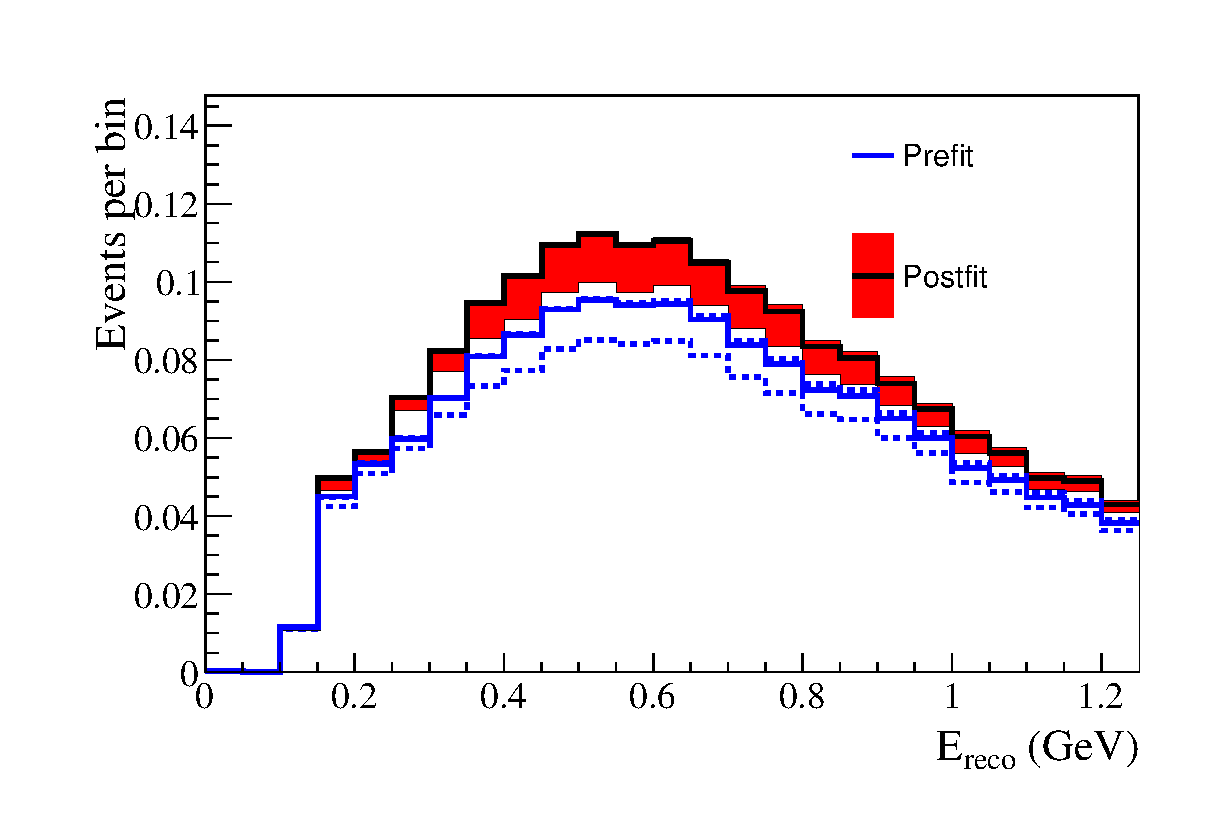
\includegraphics[width=20pc]{./nuebar_plots/spectrum_tweaked/unoscillated_Osc_param_envelope.eps}
\caption {
  Error envelopes for the energy spectrum as a result of oscillation parameters.
  \NumToys toy MC experiments were generated with randomized systematic parameters and the 1$\sigma$ spread of bin contents was calculated.
  BANFF tuned MC templates were used.
  Existing correlations between the systematic parameters were taken into account.
  The $\bar{\nu}_{\mu} \to \bar{\nu}_e$ signal is disabled setting $\beta=0$. 
  The error envelopes in each bin correspond to the $1\sigma$ error 
  obtained from the distribution of the extracted number of events.
  First the median is found. 
  Then the upper (lower) error corresponds
  to the number of events for which the 34\% of toys is contained
  in the right (left) side of the median.
  The continuos line shows the expected nominal reconstructed energy distribution 
  for pre-BANFF (blue) and post-BANFF (black).
}
\label{fig:RHC1Re_oscillated_Osc_envelope_beta0}
\end{minipage}
\hspace{0.06\linewidth}
\begin{minipage}[t]{0.48\linewidth}
\center
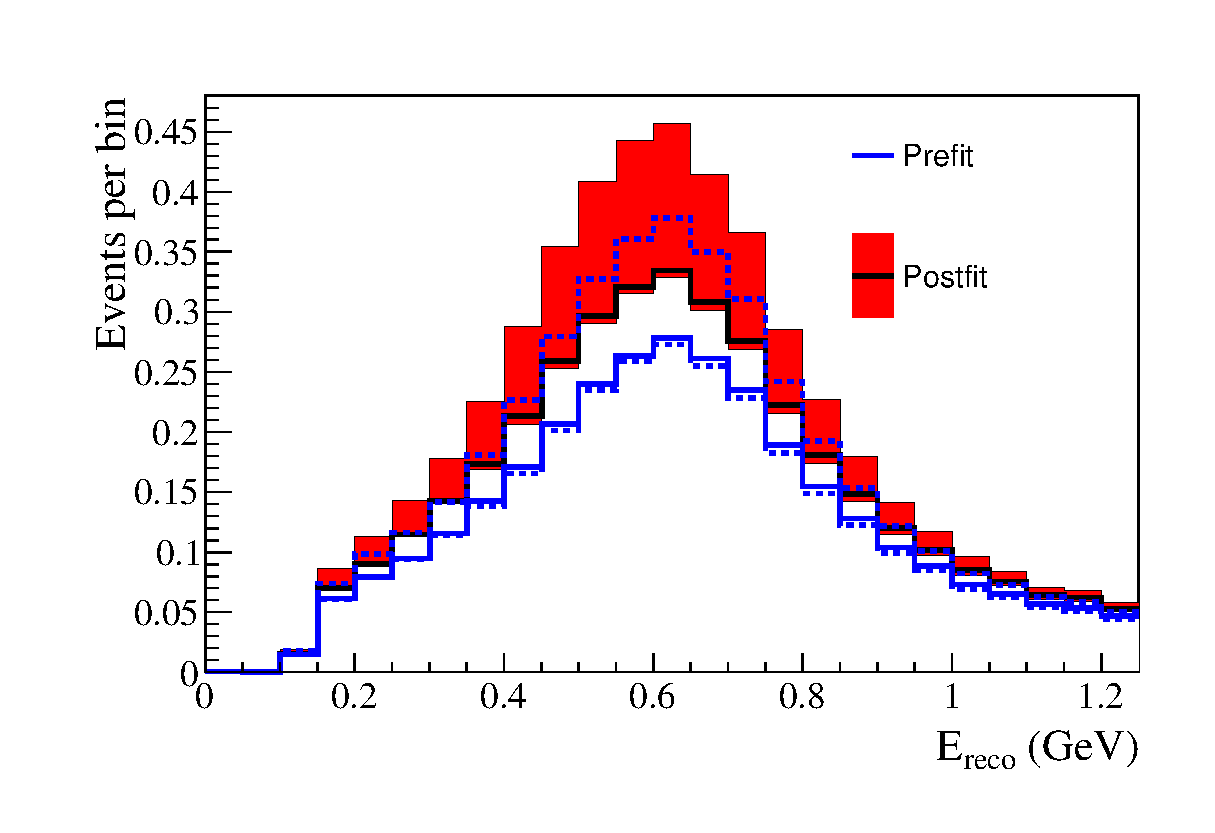
\includegraphics[width=20pc]{./nuebar_plots/spectrum_tweaked/oscillated_Osc_param_envelope.eps}
\caption {
  Error envelopes for the energy spectrum as a result of oscillation parameters.
  \NumToys toy MC experiments were generated with randomized systematic parameters and the 1$\sigma$ spread of bin contents was calculated.
  BANFF tuned MC templates were used.
  Existing correlations between the systematic parameters were taken into account.
  The $\bar{\nu}_{\mu} \to \bar{\nu}_e$ signal is enabled setting $\beta=1$. 
  The error envelopes in each bin correspond to the $1\sigma$ error 
  obtained from the distribution of the extracted number of events.
  First the median (red line) is found. 
  Then the upper (lower) error corresponds
  to the number of events for which the 34\% of toys is contained
  in the right (left) side of the median.
  The continuos line shows the expected nominal reconstructed energy distribution 
  for pre-BANFF (blue) and post-BANFF (black).
}
\label{fig:RHC1Re_oscillated_Osc_envelope_beta1}
\end{minipage}
\end{figure*}


\begin{figure*}[htb]
\begin{minipage}[t]{0.48\linewidth}
\center
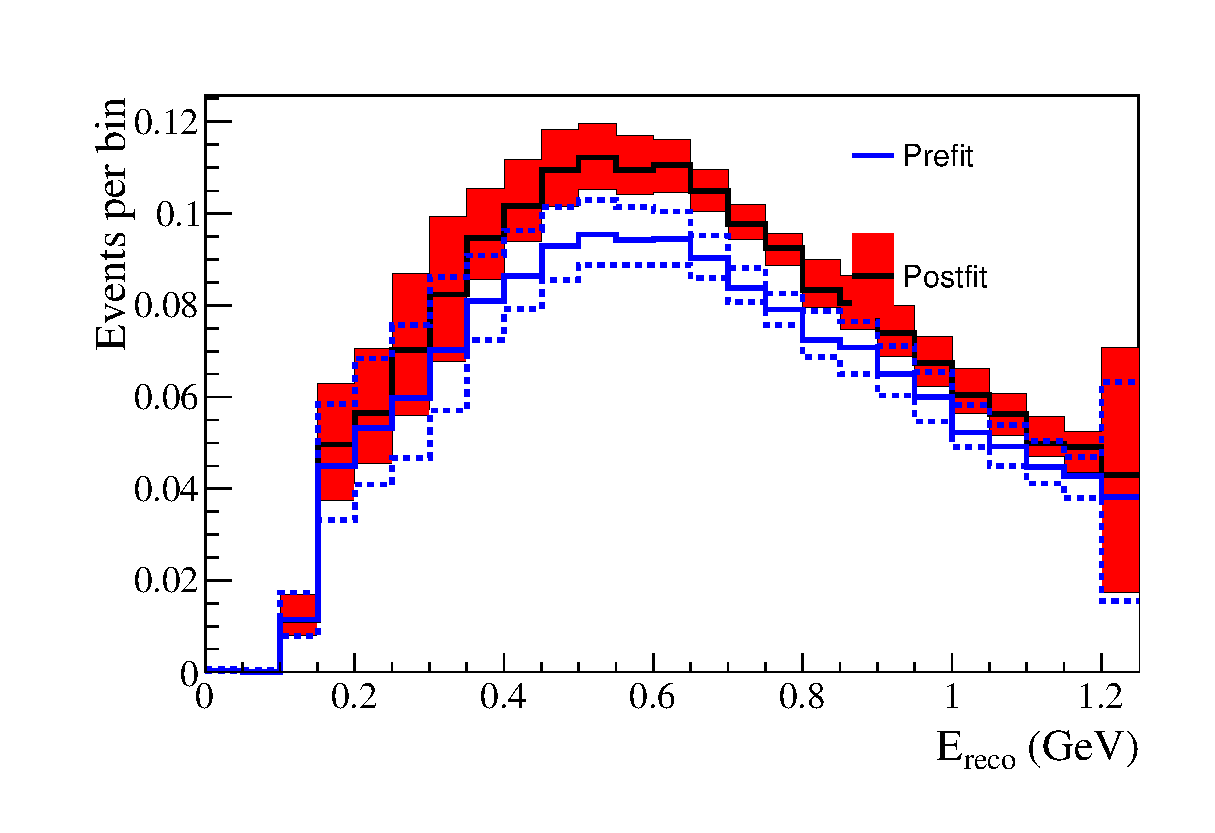
\includegraphics[width=20pc]{./nuebar_plots/spectrum_tweaked/unoscillated_SKDet_FSI_envelope.eps}
\caption {
  Error envelopes for the energy spectrum as a result of SuperK detector and FSI/SI parameters.
  \NumToys toy MC experiments were generated with randomized systematic parameters and the 1$\sigma$ spread of bin contents was calculated.
  BANFF tuned MC templates were used.
  Existing correlations between the systematic parameters were taken into account.
  The $\bar{\nu}_{\mu} \to \bar{\nu}_e$ signal is disabled setting $\beta=0$. 
  The error envelopes in each bin correspond to the $1\sigma$ error 
  obtained from the distribution of the extracted number of events.
  First the median (red line) is found. 
  Then the upper (lower) error corresponds
  to the number of events for which the 34\% of toys is contained
  in the right (left) side of the median.
  The continuos line shows the expected nominal reconstructed energy distribution 
  for pre-BANFF (blue) and post-BANFF (black).
}
\label{fig:RHC1Re_unoscillated_SKDet_FSI_envelope}
\end{minipage}
\hspace{0.06\linewidth}
\begin{minipage}[t]{0.48\linewidth}
\center
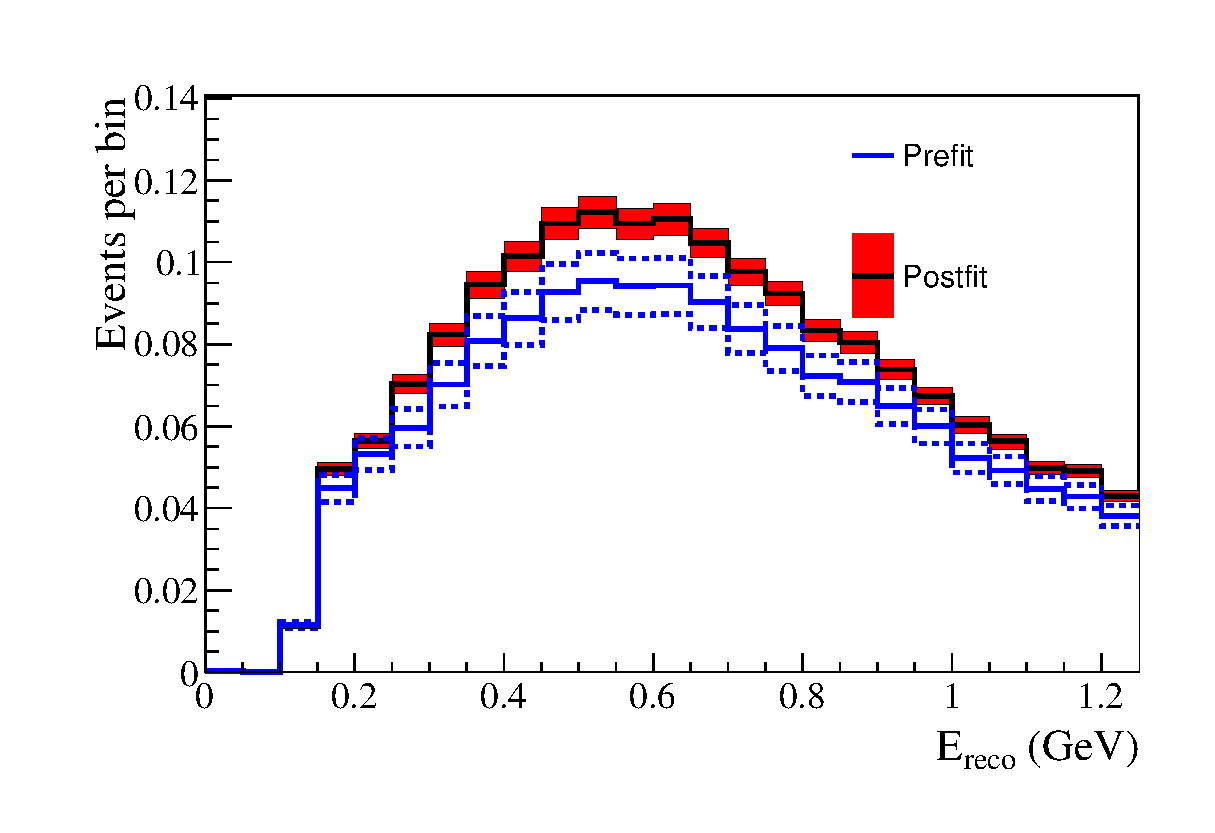
\includegraphics[width=20pc]{./nuebar_plots/spectrum_tweaked/unoscillated_BANFF_flux_envelope.eps}
\caption {
  Error envelopes for the energy spectrum as a result of BANFF flux systematics.
  \NumToys toy MC experiments were generated with randomized systematic parameters and the 1$\sigma$ spread of bin contents was calculated.
  BANFF tuned MC templates were used.
  Existing correlations between the systematic parameters were taken into account.
  The $\bar{\nu}_{\mu} \to \bar{\nu}_e$ signal is enabled setting $\beta=0$. 
  The error envelopes in each bin correspond to the $1\sigma$ error 
  obtained from the distribution of the extracted number of events.
  First the median (red line) is found. 
  Then the upper (lower) error corresponds
  to the number of events for which the 34\% of toys is contained
  in the right (left) side of the median.
  The continuos line shows the expected nominal reconstructed energy distribution 
  for pre-BANFF (blue) and post-BANFF (black).
}
\label{fig:RHC1Re_unoscillated_BANFF_flux_envelope}
\end{minipage}
\end{figure*}

\begin{figure*}[htb]
\begin{minipage}[t]{0.48\linewidth}
\center
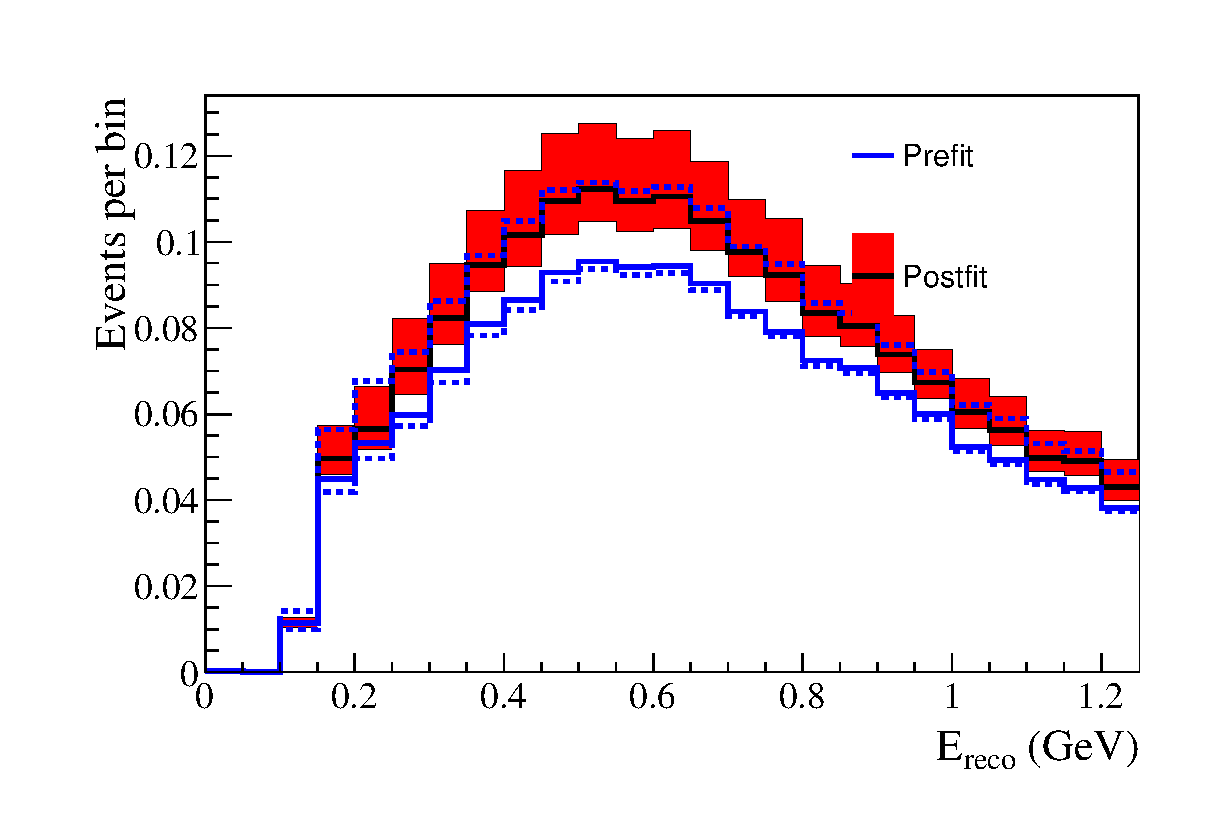
\includegraphics[width=20pc]{./nuebar_plots/spectrum_tweaked/unoscillated_BANFF_xsec_envelope.eps}
\caption {
  Error envelopes for the energy spectrum as a result of only cross-section BANFF parameters.
  \NumToys toy MC experiments were generated with randomized systematic parameters and the 1$\sigma$ spread of bin contents was calculated.
  BANFF tuned MC templates were used.
  Existing correlations between the systematic parameters were taken into account.
  The $\bar{\nu}_{\mu} \to \bar{\nu}_e$ signal is disabled setting $\beta=0$. 
  The error envelopes in each bin correspond to the $1\sigma$ error 
  obtained from the distribution of the extracted number of events.
  First the median (red line) is found. 
  Then the upper (lower) error corresponds
  to the number of events for which the 34\% of toys is contained
  in the right (left) side of the median.
  The continuos line shows the expected nominal reconstructed energy distribution 
  for pre-BANFF (blue) and post-BANFF (black).
}
\label{fig:RHC1Re_unoscillated_BANFF_xsec_envelope}
\end{minipage}
\hspace{0.06\linewidth}
\begin{minipage}[t]{0.48\linewidth}
\center
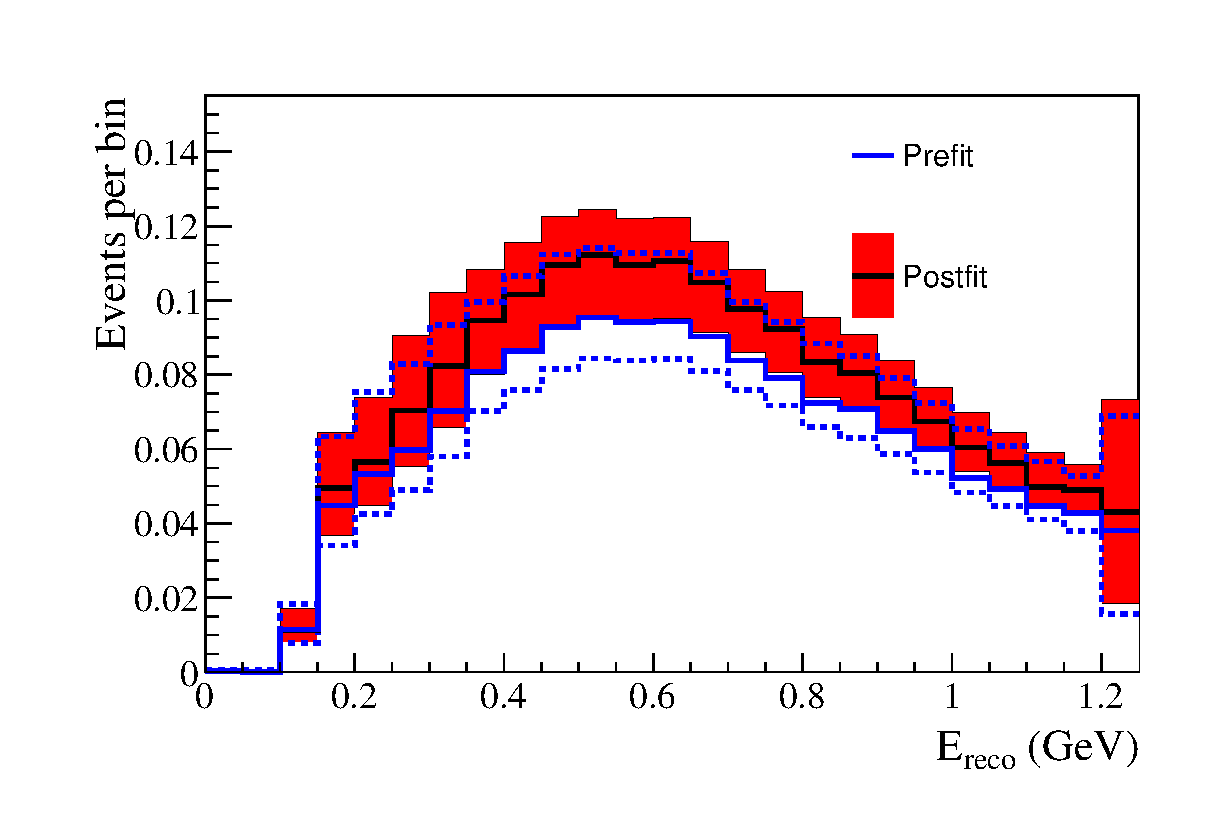
\includegraphics[width=20pc]{./nuebar_plots/spectrum_tweaked/unoscillated_all_envelope.eps}
\caption {
  Error envelopes for the energy spectrum as a result of all systematic parameters.
  \NumToys toy MC experiments were generated with randomized systematic parameters and the 1$\sigma$ spread of bin contents was calculated.
  BANFF tuned MC templates were used.
  Existing correlations between the systematic parameters were taken into account.
  The $\bar{\nu}_{\mu} \to \bar{\nu}_e$ signal is disabled setting $\beta=0$. 
  The error envelopes in each bin correspond to the $1\sigma$ error 
  obtained from the distribution of the extracted number of events.
  First the median (red line) is found. 
  Then the upper (lower) error corresponds
  to the number of events for which the 34\% of toys is contained
  in the right (left) side of the median.
  The continuos line shows the expected nominal reconstructed energy distribution 
  for pre-BANFF (blue) and post-BANFF (black).
}
\label{fig:RHC1Re_unoscillated_all_envelope}
\end{minipage}
\end{figure*}

\clearpage

\begin{figure*}[htb]
\begin{minipage}[t]{0.48\linewidth}
\center
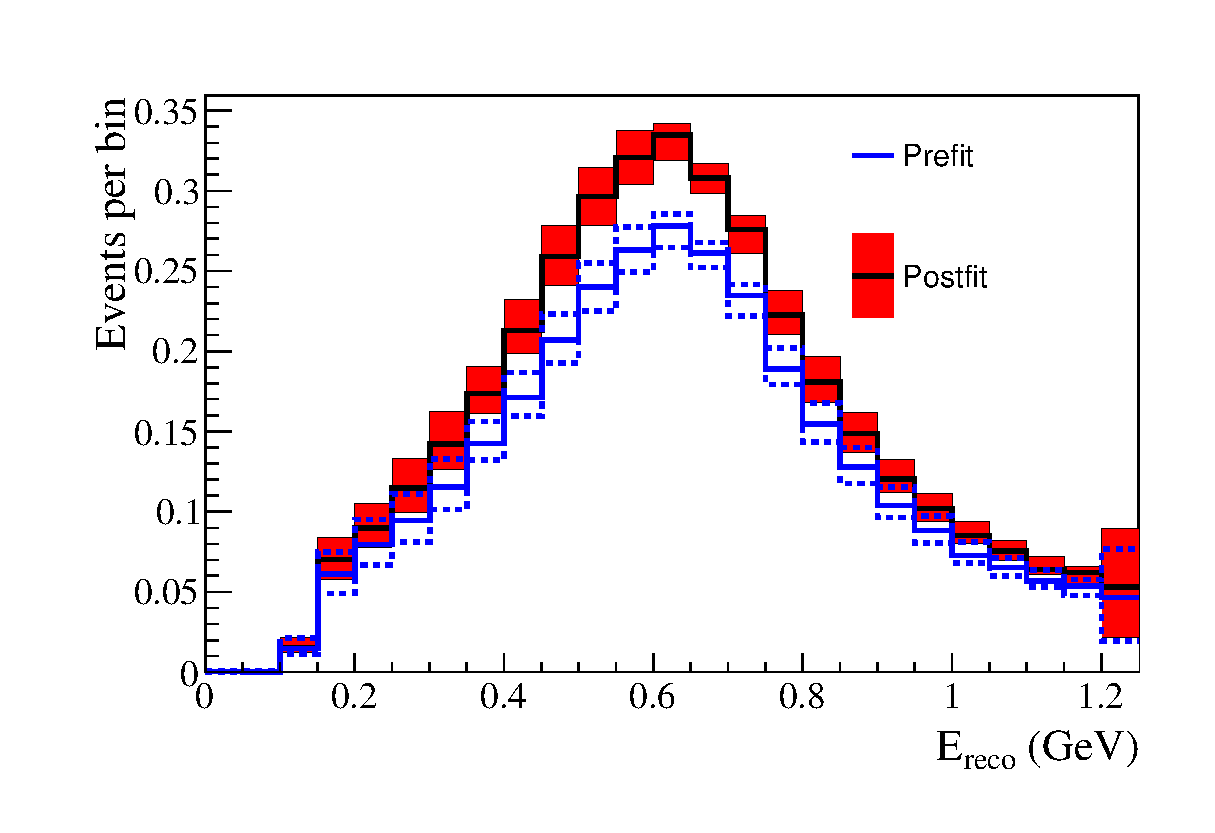
\includegraphics[width=20pc]{./nuebar_plots/spectrum_tweaked/oscillated_SKDet_FSI_envelope.eps}
\caption {
  Error envelopes for the energy spectrum as a result of SuperK detector and FSI/SI parameters.
  \NumToys toy MC experiments were generated with randomized systematic parameters and the 1$\sigma$ spread of bin contents was calculated.
  BANFF tuned MC templates were used.
  Existing correlations between the systematic parameters were taken into account.
  Oscillations were fixed to the parameter values shown in table~\ref{tab:osc_params_fixed_values_reactor}.
  The $\bar{\nu}_{\mu} \to \bar{\nu}_e$ signal is enabled setting $\beta=1$. 
  The error envelopes in each bin correspond to the $1\sigma$ error 
  obtained from the distribution of the extracted number of events.
  First the median (red line) is found. 
  Then the upper (lower) error corresponds
  to the number of events for which the 34\% of toys is contained
  in the right (left) side of the median.
  The continuos line shows the expected nominal reconstructed energy distribution 
  for pre-BANFF (blue) and post-BANFF (black).
}
\label{fig:RHC1Re_oscillated_SKDet_FSI_envelope}
\end{minipage}
\hspace{0.06\linewidth}
\begin{minipage}[t]{0.48\linewidth}
\center
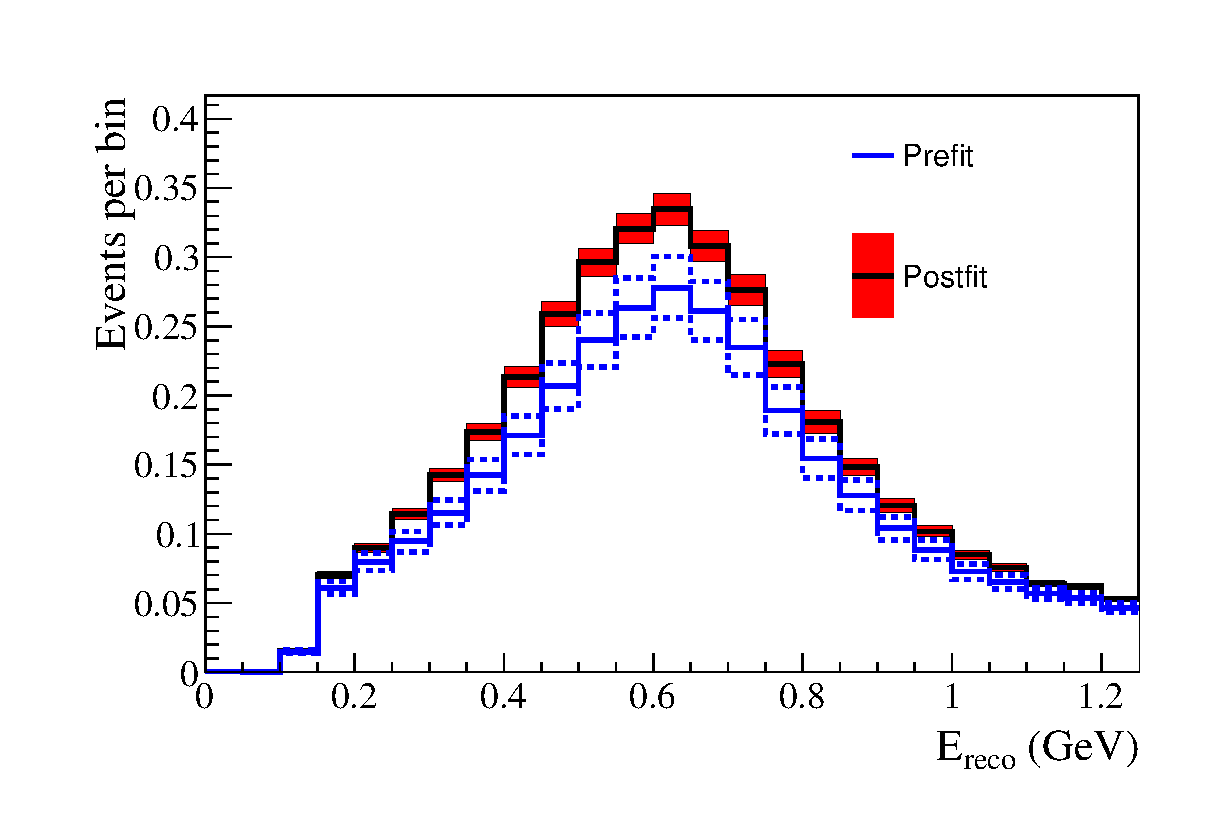
\includegraphics[width=20pc]{./nuebar_plots/spectrum_tweaked/oscillated_BANFF_flux_envelope.eps}
\caption {
  Error envelopes for the energy spectrum as a result of BANFF flux systematics.
  \NumToys toy MC experiments were generated with randomized systematic parameters and the 1$\sigma$ spread of bin contents was calculated.
  BANFF tuned MC templates were used.
  Existing correlations between the systematic parameters were taken into account.
  Oscillations were fixed to the parameter values shown in table~\ref{tab:osc_params_fixed_values_reactor}.
  The $\bar{\nu}_{\mu} \to \bar{\nu}_e$ signal is enabled setting $\beta=1$. 
  The error envelopes in each bin correspond to the $1\sigma$ error 
  obtained from the distribution of the extracted number of events.
  First the median (red line) is found. 
  Then the upper (lower) error corresponds
  to the number of events for which the 34\% of toys is contained
  in the right (left) side of the median.
  The continuos line shows the expected nominal reconstructed energy distribution 
  for pre-BANFF (blue) and post-BANFF (black).
}
\label{fig:RHC1Re_oscillated_BANFF_flux_envelope}
\end{minipage}
\end{figure*}

\begin{figure*}[htb]
\begin{minipage}[t]{0.48\linewidth}
\center
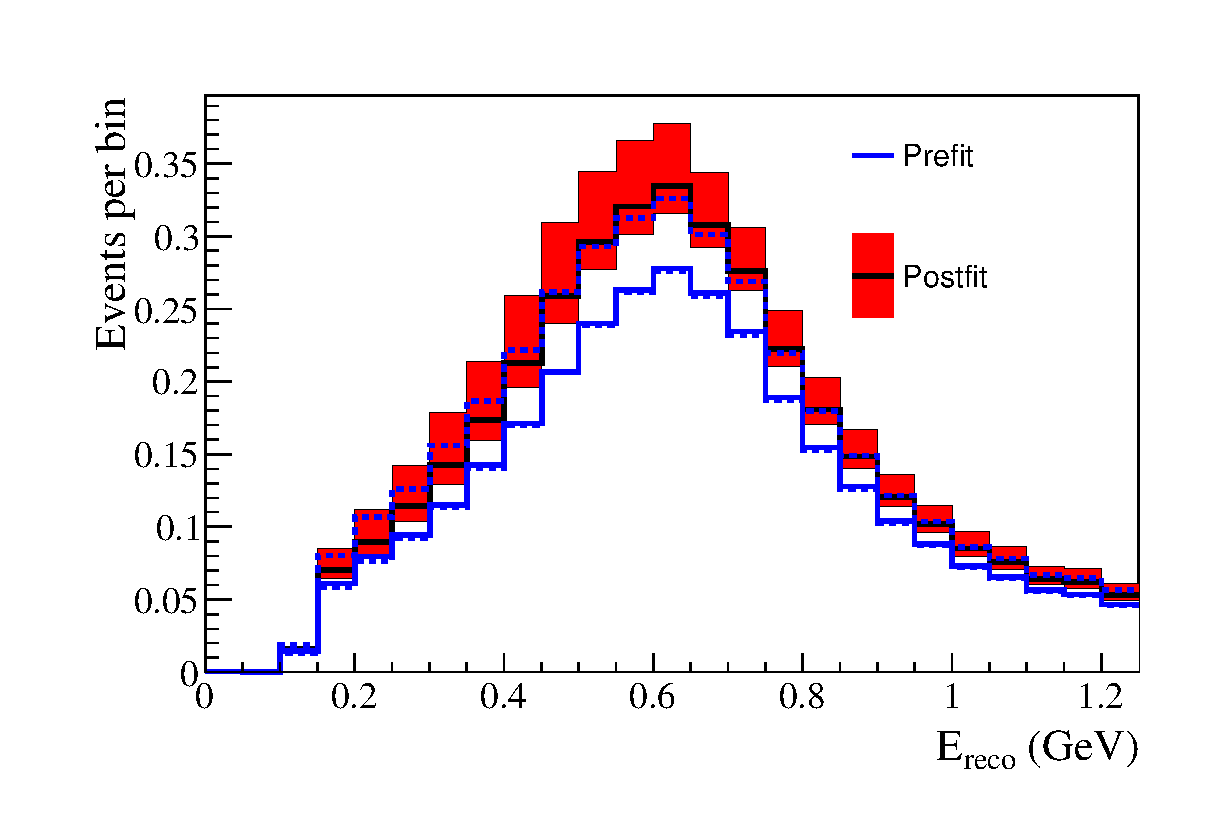
\includegraphics[width=20pc]{./nuebar_plots/spectrum_tweaked/oscillated_BANFF_xsec_envelope.eps}
\caption {
  Error envelopes for the energy spectrum as a result of only cross-section BANFF parameters.
  \NumToys toy MC experiments were generated with randomized systematic parameters and the 1$\sigma$ spread of bin contents was calculated.
  BANFF tuned MC templates were used.
  Existing correlations between the systematic parameters were taken into account.
  Oscillations were fixed to the parameter values shown in table~\ref{tab:osc_params_fixed_values_reactor}.
  The $\bar{\nu}_{\mu} \to \bar{\nu}_e$ signal is enabled setting $\beta=1$. 
  The error envelopes in each bin correspond to the $1\sigma$ error 
  obtained from the distribution of the extracted number of events.
  First the median (red line) is found. 
  Then the upper (lower) error corresponds
  to the number of events for which the 34\% of toys is contained
  in the right (left) side of the median.
  The continuos line shows the expected nominal reconstructed energy distribution 
  for pre-BANFF (blue) and post-BANFF (black).
}
\label{fig:RHC1Re_oscillated_BANFF_xsec_envelope}
\end{minipage}
\hspace{0.06\linewidth}
\begin{minipage}[t]{0.48\linewidth}
\center
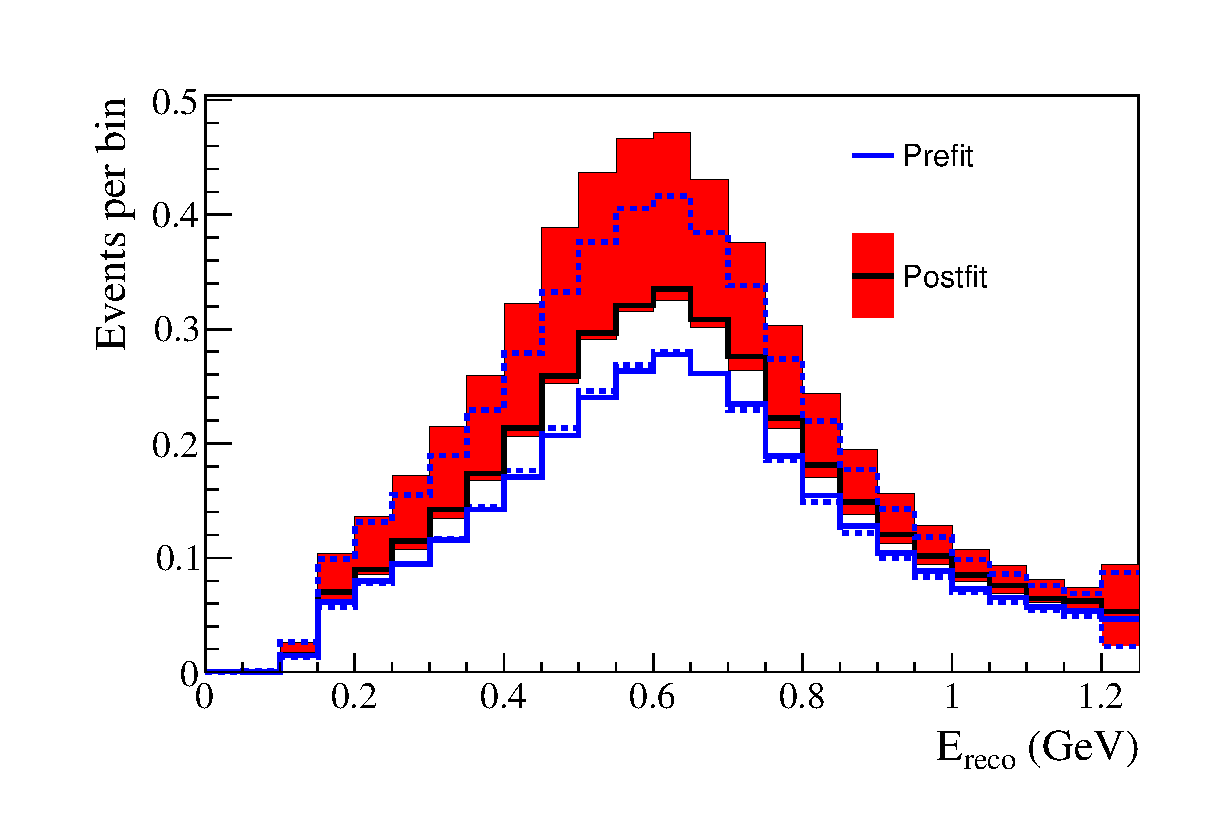
\includegraphics[width=20pc]{./nuebar_plots/spectrum_tweaked/oscillated_all_envelope.eps}
\caption {
  Error envelopes for the energy spectrum as a result of all systematic parameters.
  \NumToys toy MC experiments were generated with randomized systematic parameters and the 1$\sigma$ spread of bin contents was calculated.
  BANFF tuned MC templates were used.
  Existing correlations between the systematic parameters were taken into account.
  Oscillations were treated as shown in table~\ref{tab:osc_params_fixed_values_reactor}:
  $\sin^2 \theta_{23}$, $\sin^2 \theta_{13}$, $\Delta m^2_{23}$ and $\delta_{CP}$ were randomly extracted.
  The $\bar{\nu}_{\mu} \to \bar{\nu}_e$ signal is enabled setting $\beta=1$. 
  The error envelopes in each bin correspond to the $1\sigma$ error 
  obtained from the distribution of the extracted number of events.
  First the median (red line) is found. 
  Then the upper (lower) error corresponds
  to the number of events for which the 34\% of toys is contained
  in the right (left) side of the median.
  The continuos line shows the expected nominal reconstructed energy distribution 
  for pre-BANFF (blue) and post-BANFF (black).
}
\label{fig:RHC1Re_oscillated_all_envelope}
\end{minipage}
\end{figure*}



\clearpage




%Ratio oscillated

In Figs.~\ref{fig:RHC1Re_oscillated_SKDet_FSI_envelope_ratio} to ~\ref{fig:RHC1Re_oscillated_all_envelope_ratio}
the error envelopes, expressed as a ratio of event count, for the energy spectrum as a result of oscillation parameters,
SK detector and FSI/SI systematics, BANFF flux systematics, BANFF cross section systematics and 
all the systematic parameters.


\begin{figure*}[htb]
\center
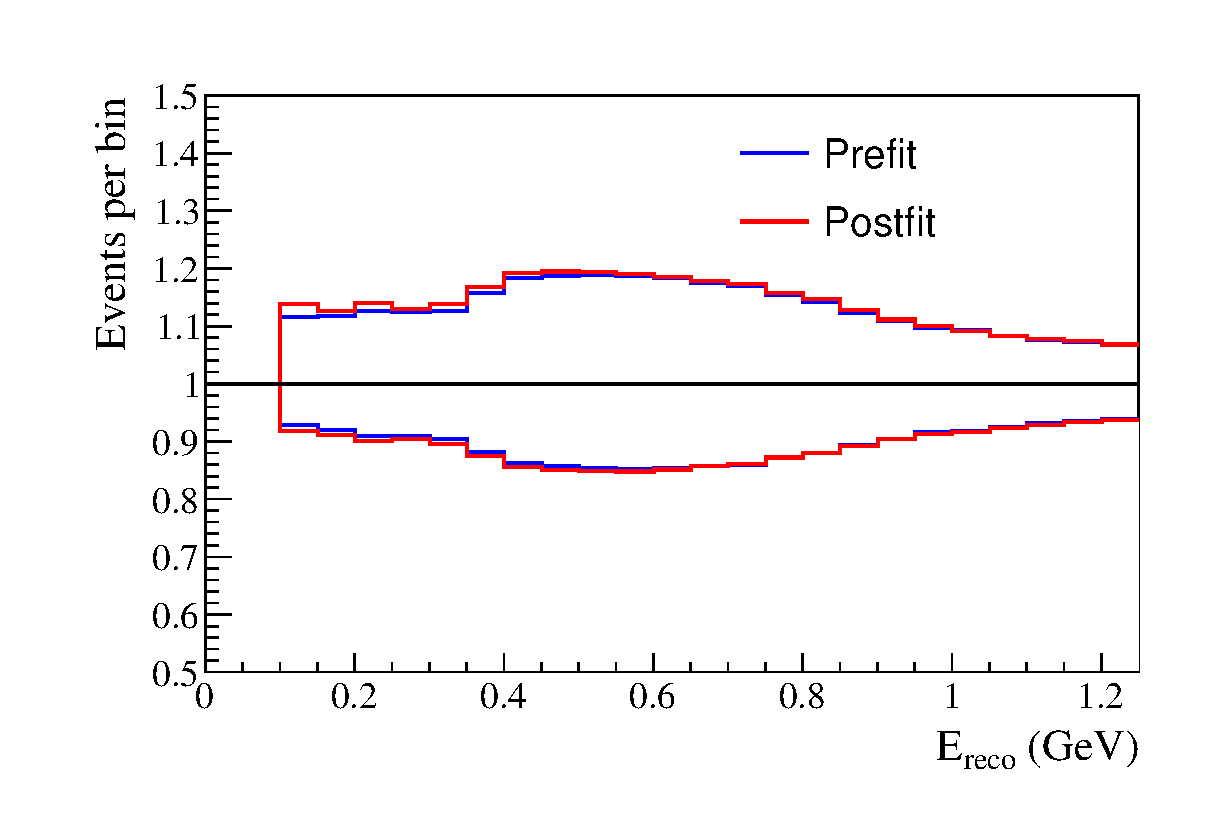
\includegraphics[width=20pc]{./nuebar_plots/spectrum_tweaked/oscillated_Osc_param_envelope_ratio.eps}
%
\includegraphics[width=20pc]{./images/missing_plot-eps-converted-to.pdf}
\caption {
  Error envelopes, expressed as a ratio of event count, for the energy spectrum as a result of oscillation parameters.
  \NumToys toy MC experiments were generated with randomized systematic parameters and the 1$\sigma$ spread of bin contents was calculated.
  BANFF tuned MC templates were used.
  All systematic parameters were considered and their correlations were taken into account.
  Oscillations were applied with the parameter values shown in table~\ref{tab:osc_params_fixed_values_reactor}.
  The fractional error in each bin corresponds to the $1\sigma$ error 
  obtained from the distribution of the extracted number of events.
  First the median is found. 
  Then the upper (lower) error corresponds
  to the number of events for which the 34\% of toys is contained
  in the right (left) side of the median.
  The continuos line shows the pre-BANFF (blue) and post-BANFF (red) ratios.
}
\label{fig:RHC1Re_oscillated_SKDet_FSI_envelope_ratio}
\end{figure*}


\begin{figure*}[htb]
\begin{minipage}[t]{0.48\linewidth}
\center
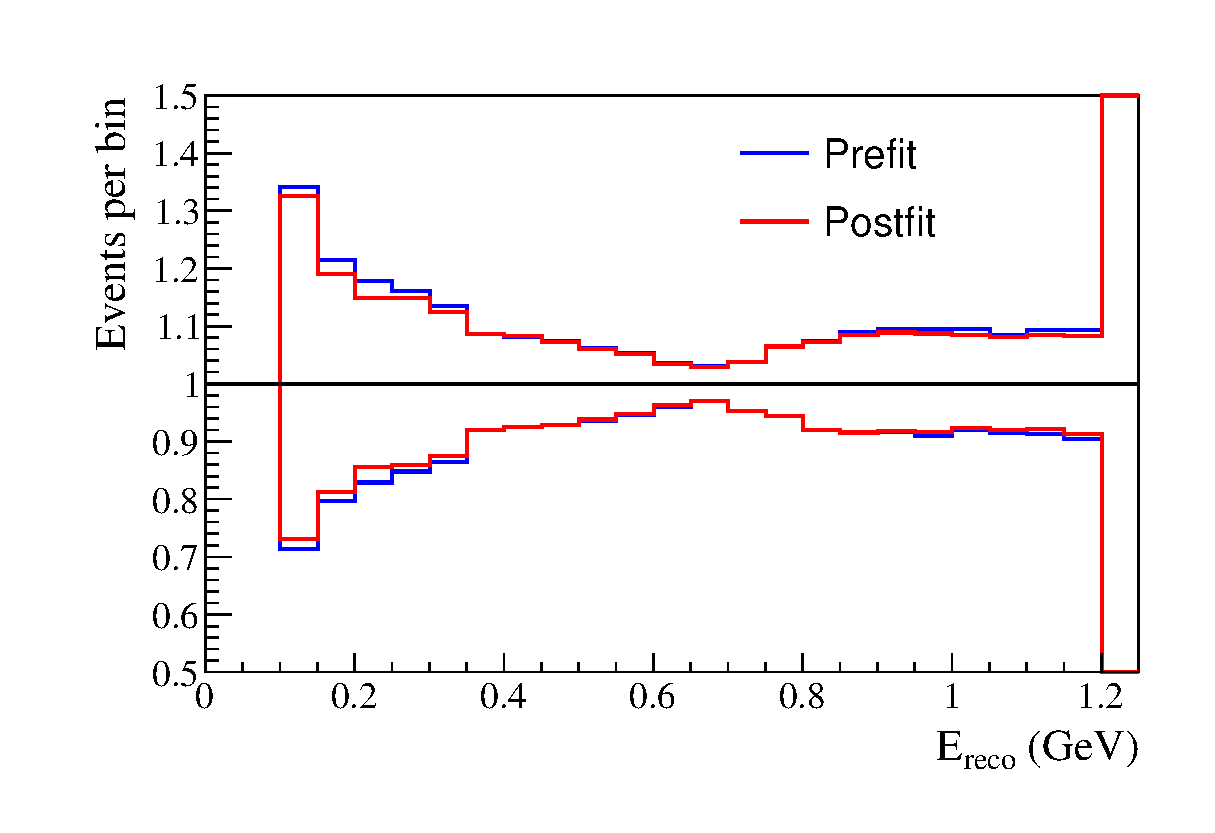
\includegraphics[width=20pc]{./nuebar_plots/spectrum_tweaked/oscillated_SKDet_FSI_envelope_ratio.eps}
%
\includegraphics[width=20pc]{./images/missing_plot-eps-converted-to.pdf}
\caption {
  Error envelopes, expressed as a ratio of event count, for the energy spectrum as a result of SuperK detector and FSI/SI parameters.
  \NumToys toy MC experiments were generated with randomized systematic parameters and the 1$\sigma$ spread of bin contents was calculated.
  BANFF tuned MC templates were used.
  All systematic parameters were considered and their correlations were taken into account.
  Oscillations were applied with the parameter values shown in table~\ref{tab:osc_params_fixed_values_reactor}.
  The fractional error in each bin corresponds to the $1\sigma$ error 
  obtained from the distribution of the extracted number of events.
  First the median (red line) is found. 
  Then the upper (lower) error corresponds
  to the number of events for which the 34\% of toys is contained
  in the right (left) side of the median.
  The continuos line shows the pre-BANFF (blue) and post-BANFF (red) ratios.
}
\label{fig:RHC1Re_oscillated_SKDet_FSI_envelope_ratio}
\end{minipage}
\hspace{0.06\linewidth}
\begin{minipage}[t]{0.48\linewidth}
\center
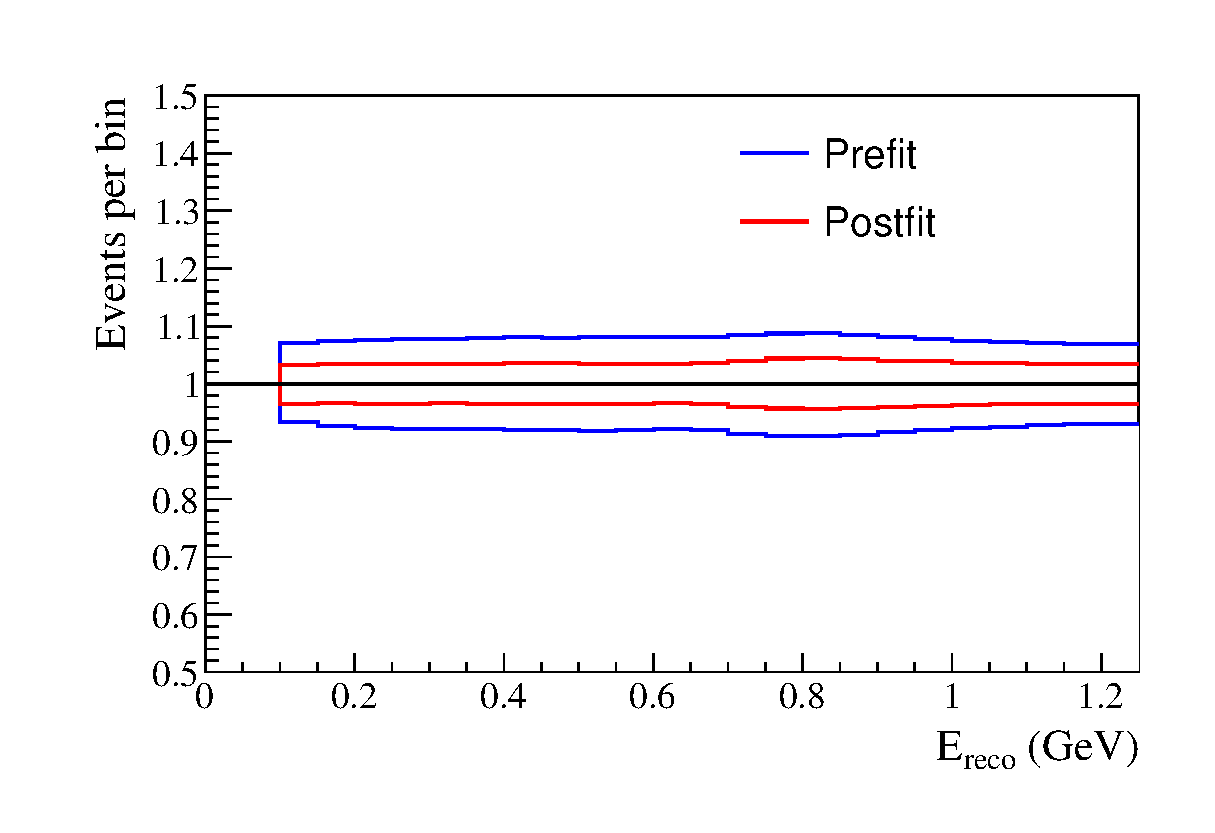
\includegraphics[width=20pc]{./nuebar_plots/spectrum_tweaked/oscillated_BANFF_flux_envelope_ratio.eps}
%
\includegraphics[width=20pc]{./images/missing_plot-eps-converted-to.pdf}
\caption {
  Error envelopes, expressed as a ratio of event count, for the energy spectrum as a result of BANFF flux systematics.
  \NumToys toy MC experiments were generated with randomized systematic parameters and the 1$\sigma$ spread of bin contents was calculated.
  BANFF tuned MC templates were used.
  All systematic parameters were considered and their correlations were taken into account.
  Oscillations were applied with the parameter values shown in table~\ref{tab:osc_params_fixed_values_reactor}.
  The fractional error in each bin corresponds to the $1\sigma$ error 
  obtained from the distribution of the extracted number of events.
  First the median (red line) is found. 
  Then the upper (lower) error corresponds
  to the number of events for which the 34\% of toys is contained
  in the right (left) side of the median.
  The continuos line shows the pre-BANFF (blue) and post-BANFF (red) ratios.
}
\label{fig:RHC1Re_oscillated_BANFF_flux_envelope_ratio}
\end{minipage}
\end{figure*}

\begin{figure*}[htb]
\begin{minipage}[t]{0.48\linewidth}
\center
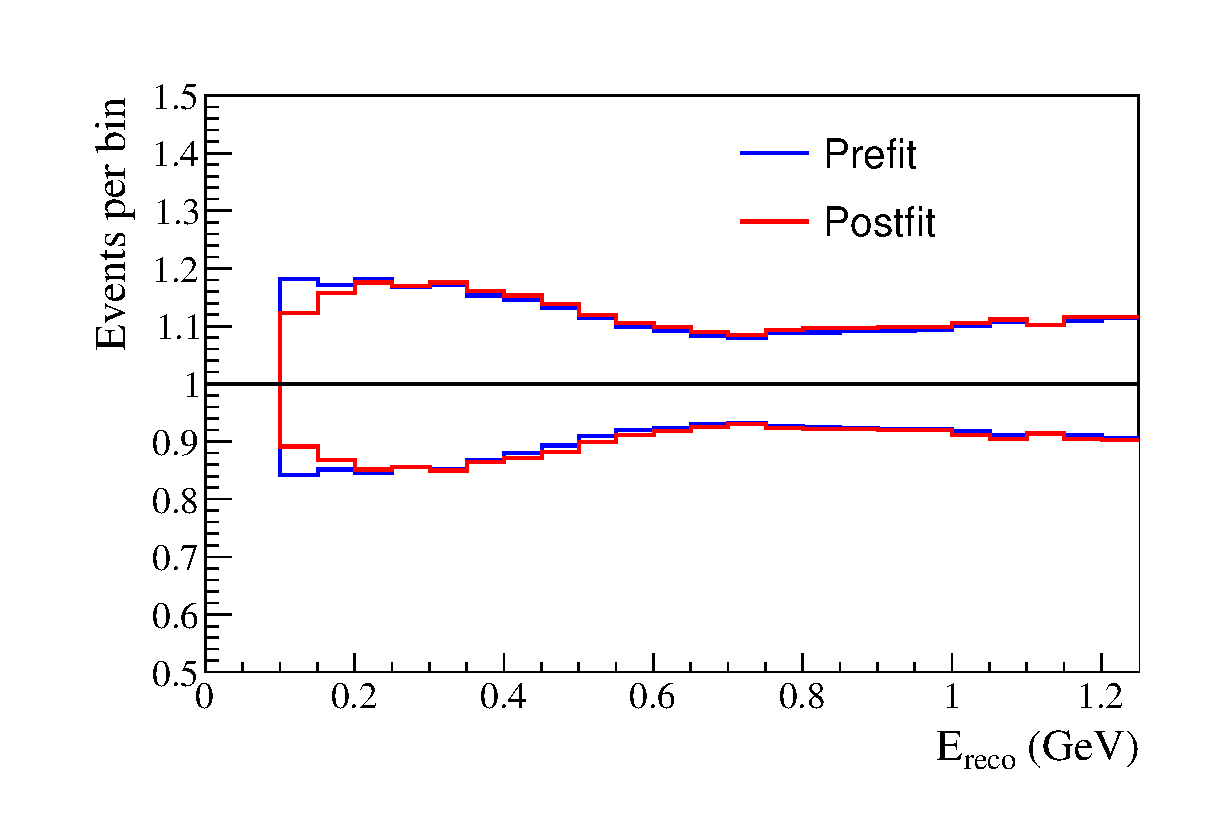
\includegraphics[width=20pc]{./nuebar_plots/spectrum_tweaked/oscillated_BANFF_xsec_envelope_ratio.eps}
%
\includegraphics[width=20pc]{./images/missing_plot-eps-converted-to.pdf}
\caption {
  Error envelopes, expressed as a ratio of event count, for the energy spectrum as a result of only cross-section BANFF parameters.
  \NumToys toy MC experiments were generated with randomized systematic parameters and the 1$\sigma$ spread of bin contents was calculated.
  BANFF tuned MC templates were used.
  All systematic parameters were considered and their correlations were taken into account.
  Oscillations were applied with the parameter values shown in table~\ref{tab:osc_params_fixed_values_reactor}.
  The fractional error in each bin corresponds to the $1\sigma$ error 
  obtained from the distribution of the extracted number of events.
  First the median (red line) is found. 
  Then the upper (lower) error corresponds
  to the number of events for which the 34\% of toys is contained
  in the right (left) side of the median.
  The continuos line shows the pre-BANFF (blue) and post-BANFF (red) ratios.
}
\label{fig:RHC1Re_oscillated_BANFF_xsec_envelope_ratio}
\end{minipage}
\hspace{0.06\linewidth}
\begin{minipage}[t]{0.48\linewidth}
\center
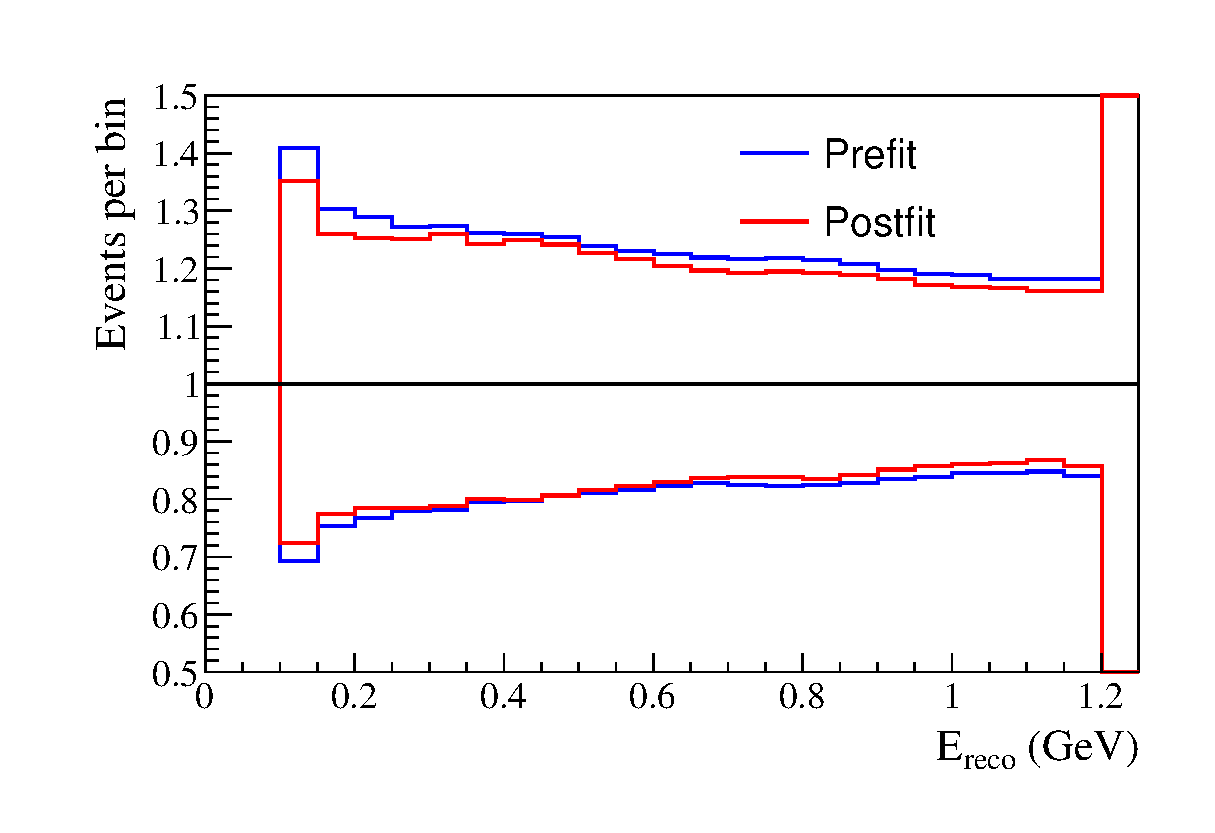
\includegraphics[width=20pc]{./nuebar_plots/spectrum_tweaked/oscillated_all_envelope_ratio.eps}
%
\includegraphics[width=20pc]{./images/missing_plot-eps-converted-to.pdf}
\caption {
  Error envelopes, expressed as a ratio of event count, for the energy spectrum as a result of all systematic parameters.
  \NumToys toy MC experiments were generated with randomized systematic parameters and the 1$\sigma$ spread of bin contents was calculated.
  BANFF tuned MC templates were used.
  All systematic parameters were considered and their correlations were taken into account.
  Oscillations were applied with the parameter values shown in table~\ref{tab:osc_params_fixed_values_reactor}.
  The fractional error in each bin corresponds to the $1\sigma$ error 
  obtained from the distribution of the extracted number of events.
  First the median (red line) is found. 
  Then the upper (lower) error corresponds
  to the number of events for which the 34\% of toys is contained
  in the right (left) side of the median.
  The continuos line shows the pre-BANFF (blue) and post-BANFF (red) ratios.
}
\label{fig:RHC1Re_oscillated_all_envelope_ratio}
\end{minipage}
\end{figure*}


% ..................

\begin{table}[htb]
\centering
\begin{tabular}{| c | D{.}{.}{-1} | D{.}{.}{-1} |}
\hline
%  {\bf Source of uncertainty}    & \multicolumn{1}{c|}{{\bf ${\delta}N_{SK}$/$N_{SK}$}} & \multicolumn{1}{c|}{{\bf ${\delta}N_{SK}$/$N_{SK}$}}\\
  {\bf Source of uncertainty}    & \multicolumn{1}{c|}{{\bf ${\delta}N_{SK}$/$ <N_{SK} >$}} & \multicolumn{1}{c|}{{\bf ${\delta}N_{SK}$/$<N_{SK}>$}}\\
                                 & \multicolumn{1}{c|}{($\beta=0$)} & \multicolumn{1}{c|}{($\beta=1$)}\\
\hline
  SuperK detector    				& 5.05\%                         & 3.03\%                        \\
  FSI + SI + PN 					& 4.34\%				& 2.45\%			\\
  SuperK detector + FSI + SI + PN     & 6.66\%                         & 3.90\%                        \\
\hline
  BANFF (prefit)                 &  12.37\%                        & 12.91\%                       \\
  BANFF (postfit)                & 9.72\%                         & 10.29\%                        \\
\hline
  BANFF (Non-oxygen, postfit)    	& 3.40\%         	         & 3.02\%                        \\
  BANFF (Oxygen-specific postfit) 	& 9.24\%                    & 10.14\%                        \\
  MEC (Oxygen-specific postfit)	   	& 8.86\%                        	 & 9.28\%                        \\
\hline
  Oscillation parameters         & 4.72\%                         & 13.38\%                       \\
\hline
  Total (BANFF prefit)           &  14.96\%                        & 18.60\%                       \\
  Total (BANFF postfit)          & 12.75\%                         & 17.21\%                       \\
\hline
\end{tabular}
\caption{
 Effect of 1$\sigma$ variations of the groups of systematics parameters on total number of
 1-ring electron-like events in the reverse-horn current sample.
 The BANFF parameters considered to be oxygen-specific are Oxygen MEC normalisation, Fermi Energy, Binding Energy, CC Coherent Normalisation,
 NC Coherent normalization and the nue/numu normalisation. 
The effect of each group of systematics is computed as the standard deviation divided by the mean of the distribution
of the total number of superK events.
\NumToys are performed.
% \newline
%{\bf TO UPDATE}
%\newline
}
\label{tab:nsk_systematic_table_summary}
\end{table}

%\input{./tables/nsk_systematic_table_summary_PROVA.tex}

%..................

\begin{table}
\centering
\begin{tabular}{| c || D{.}{.}{-1} | D{.}{.}{-1} || D{.}{.}{-1} | D{.}{.}{-1} |}
\hline
  Source of uncertainty        &  \multicolumn {2}{c||}{${\delta}N_{SK}$/$N_{SK}$} & \multicolumn {2}{c|}{${\delta}N_{SK}$/$N_{SK}$} \\
                               &  \multicolumn {2}{c||}{(no oscillation)}          & \multicolumn {2}{c|}{(oscillations with typical params)} \\
                               & \multicolumn {1}{c|}{BANFF prefit} & \multicolumn {1}{c||}{BANFF postfit} & \multicolumn {1}{c|}{BANFF prefit} & \multicolumn {1}{c|}{BANFF postfit} \\
\hline
               $f_{E; r}^{SK}$ &               0 &               0 &               0 &               0  \\   
           $f_{0; r}^{SK+FSI}$ &            0.09 &           0.098 &            0.15 &            0.18  \\   
           $f_{1; r}^{SK+FSI}$ &             1.8 &             1.9 &            0.68 &            0.74  \\   
           $f_{2; r}^{SK+FSI}$ &             0.4 &            0.43 &            0.92 &             1.0  \\   
           $f_{3; r}^{SK+FSI}$ &             2.4 &             2.1 &             4.6 &             4.0  \\   
           $f_{4; r}^{SK+FSI}$ &           0.017 &           0.016 &            0.25 &            0.27  \\   
           $f_{5; r}^{SK+FSI}$ &             1.1 &             0.9 &             3.8 &             3.2  \\   
\hline
         $f_{0; t, r}^{banff}$ &            0.36 &            0.27 &            0.85 &            0.66  \\   
         $f_{1; t, r}^{banff}$ &             1.0 &            0.74 &            0.67 &             0.5  \\   
         $f_{2; t, r}^{banff}$ &             1.9 &             1.3 &            0.12 &           0.085  \\   
         $f_{3; t, r}^{banff}$ &             2.3 &             1.6 &             0.3 &            0.22  \\   
         $f_{4; t, r}^{banff}$ &             3.4 &             2.4 &             2.2 &             1.6  \\   
         $f_{5; t, r}^{banff}$ &             1.0 &            0.66 &             1.8 &             1.2  \\   
         $f_{6; t, r}^{banff}$ &            0.63 &            0.39 &             1.7 &             1.1  \\   
         $f_{7; t, r}^{banff}$ &            0.33 &             0.2 &             1.0 &            0.65  \\   
         $f_{8; t, r}^{banff}$ &            0.41 &            0.22 &             1.3 &            0.74  \\   
         $f_{9; t, r}^{banff}$ &            0.19 &           0.077 &            0.65 &            0.27  \\   
        $f_{10; t, r}^{banff}$ &           0.051 &           0.019 &            0.17 &           0.066  \\   
        $f_{11; t, r}^{banff}$ &           0.061 &            0.05 &           0.035 &            0.03  \\   
        $f_{12; t, r}^{banff}$ &           0.061 &           0.049 &           0.049 &            0.04  \\   
        $f_{13; t, r}^{banff}$ &           0.085 &           0.067 &            0.16 &            0.13  \\   
        $f_{14; t, r}^{banff}$ &             0.1 &            0.08 &            0.27 &            0.22  \\   
        $f_{15; t, r}^{banff}$ &           0.078 &            0.06 &            0.25 &             0.2  \\   
        $f_{16; t, r}^{banff}$ &            25.0 &             3.4 &            18.0 &             2.8  \\   
        $f_{17; t, r}^{banff}$ &             2.8 &             1.1 &             6.7 &             2.4  \\   
        $f_{18; t, r}^{banff}$ &             7.9 &             5.9 &             4.2 &             3.3  \\   
        $f_{19; t, r}^{banff}$ &             1.4 &            0.55 &             3.9 &             1.6  \\   
        $f_{20; t, r}^{banff}$ &            0.36 &            0.16 &             1.2 &            0.53  \\   
        $f_{21; t, r}^{banff}$ &             3.7 &             1.5 &             4.9 &             2.0  \\   
        $f_{22; t, r}^{banff}$ &             1.7 &            0.47 &             5.4 &             1.6  \\   
\hline
                $f_{pF; t, r}$ &           0.063 &           0.065 &            0.13 &            0.13  \\   
                $f_{SF; t, r}$ &            0.82 &            0.82 &            0.24 &            0.26  \\   
            $f_{Wshape; t, r}$ &            0.12 &           0.072 &             0.4 &            0.26  \\   
        $f_{CCothShape; t, r}$ &            0.28 &             0.3 &            0.78 &            0.89  \\   
    $f_{\pi-less\Delta; t, r}$ &             3.2 &             2.6 &             5.6 &             4.5  \\   
             $f_{bindE; t, r}$ &             0.5 &            0.43 &            0.24 &             0.2  \\   
                $f_{CCcoh; t}$ &            0.54 &            0.58 &            0.81 &            0.93  \\   
           $f_{NC1\pi^\pm; t}$ &            0.31 &            0.21 &             1.1 &            0.75  \\   
                $f_{NCoth; t}$ &            0.25 &            0.24 &            0.85 &            0.85  \\   
              $f_{CC\nu_e; t}$ &         0.00051 &          0.0005 &          0.0077 &          0.0081  \\   
          $f_{CC\bar{\nu}; t}$ &            0.61 &            0.61 &             1.2 &             1.2  \\   
\hline
         $\sin^2(\theta_{13})$ &               0 &               0 &           0.070 &           0.078  \\   
         $\sin^2(\theta_{12})$ &               0 &               0 &           0.040 &           0.036  \\   
             $\Delta m^2_{21}$ &               0 &               0 &           0.027 &           0.025  \\   
                 $\delta_{CP}$ &               0 &               0 &            0.21 &            0.19  \\   

 


\hline
\end{tabular}
\caption{
  Effects of 1$\sigma$ systematic parameter variations on
  the number of 1 $\mu$-like ring events,
  computed
  for no oscillations and
  for oscillations with
  $\sin^{2}\theta_{23}$=0.5, $|\Delta m^{2}_{32}|$=2.4$\times$10$^{-3}$ eV$^{2}$/c$^{4}$, the values shown in Tab.\
  \ref{tab:pdg2012non23} for $\sin^{2}\theta_{13}$, $\sin^{2}\theta_{12}$ and $\Delta m^{2}_{21}$,
  and $\delta_{CP}$=0. Correlations are ignored for this table. The normal mass hierarchy is assumed.
  The numbers shown were calculated for an exposure of 6.5700$\times$10$^{20}$ POT and BANFF-tuned MC templates were used.
}
\label{tab:nsk_systematic_table}
\end{table}


%..................

%\begin{table}
\small
\centering
\begin{tabular}{| c | c | c |}
\hline
 Parameter               &  $\frac{\delta_{syst} sin^2\overline{\theta_{23}}}{\delta_{stat} sin^2\overline{\theta_{23}}}$   &  $\frac{\delta_{syst}|\overline{\Delta m^2_{32}}| (eV^{2}/c^{4})}{\delta_{stat} |\overline{\Delta m^2_{32}}| (eV^{2}/c^{4})}$ \\
\hline
                               SKDet + FSI/SI  5; $E_r$ =  0.00 - 30.00 GeV; all NC; RHC & 1.040 & 0.225 \\ \hline 
                                       Meson exchange current normalisation for $^{16}$O & 0.918 & 0.127 \\ \hline 
                                                  CC coherent for $^{16}$O normalisation & 0.491 & 0.028 \\ \hline 
                            C$^{A}_{5}$ nucleon to $\Delta$ transition axial form factor & 0.422 & 0.024 \\ \hline 
                                                                    SK energy scale; RHC & 0.383 & 0.101 \\ \hline 
                                                                  NC other normalisation & 0.347 & 0.029 \\ \hline 
                               RHC $\bar{\nu_\mu}$ flux normalisation, E = 0.7 - 1.0 GeV & 0.326 & 0.048 \\ \hline 
       SKDet + FSI/SI  3; $E_r$ =  0.00 - 30.00 GeV; $\overset{(-)}{\nu_\mu}$ CCnQE; RHC & 0.315 & 0.022 \\ \hline 
                                             Scale of isospin 1/2 nonresonant background & 0.315 & 0.012 \\ \hline 
                                          Resonance-production axial-mass scaling factor & 0.247 & 0.011 \\ \hline 
                                                             Fermi momentum for $^{16}$O & 0.230 & 0.024 \\ \hline 
                               RHC $\bar{\nu_\mu}$ flux normalisation, E = 0.0 - 0.4 GeV & 0.228 & 0.021 \\ \hline 
         SKDet + FSI/SI  1; $E_r$ =  0.40 - 1.10 GeV; $\overset{(-)}{\nu_\mu}$ CCQE; RHC & 0.225 & 0.023 \\ \hline 
            SKDet + FSI/SI  4; $E_r$ =  0.00 - 30.00 GeV; $\overset{(-)}{\nu_e}$ CC; RHC & 0.211 & 0.009 \\ \hline 
                               RHC $\bar{\nu_\mu}$ flux normalisation, E = 1.0 - 1.5 GeV & 0.202 & 0.016 \\ \hline 
                                                          CCQE axial-mass scaling factor & 0.200 & 0.021 \\ \hline 
                               RHC $\bar{\nu_\mu}$ flux normalisation, E = 0.4 - 0.5 GeV & 0.190 & 0.030 \\ \hline 
                                     RHC $\nu_\mu$ flux normalisation, E = 1.0 - 1.5 GeV & 0.150 & 0.009 \\ \hline 
                               RHC $\bar{\nu_\mu}$ flux normalisation, E = 0.6 - 0.7 GeV & 0.142 & 0.009 \\ \hline 
         SKDet + FSI/SI  0; $E_r$ =  0.00 - 0.40 GeV; $\overset{(-)}{\nu_\mu}$ CCQE; RHC & 0.116 & 0.006 \\ \hline 
                               RHC $\bar{\nu_\mu}$ flux normalisation, E = 0.5 - 0.6 GeV & 0.115 & 0.025 \\ \hline 
                                     RHC $\nu_\mu$ flux normalisation, E = 0.7 - 1.0 GeV & 0.113 & 0.006 \\ \hline 
                               RHC $\bar{\nu_\mu}$ flux normalisation, E = 1.5 - 2.5 GeV & 0.108 & 0.005 \\ \hline 
                                     RHC $\nu_\mu$ flux normalisation, E = 0.0 - 0.7 GeV & 0.100 & 0.009 \\ \hline 
                                                                          CC other shape & 0.096 & 0.003 \\ \hline 
                                     RHC $\nu_\mu$ flux normalisation, E = 1.5 - 2.5 GeV & 0.087 & 0.006 \\ \hline 
                                    RHC $\nu_\mu$ flux normalisation, E = 2.5 - 30.0 GeV & 0.085 & 0.004 \\ \hline 
        SKDet + FSI/SI  2; $E_r$ =  1.10 - 30.00 GeV; $\overset{(-)}{\nu_\mu}$ CCQE; RHC & 0.070 & 0.005 \\ \hline 
                                                             Binding energy for $^{16}$O & 0.063 & 0.007 \\ \hline 
                               RHC $\bar{\nu_\mu}$ flux normalisation, E = 2.5 - 3.5 GeV & 0.051 & 0.001 \\ \hline 
                               RHC $\bar{\nu_\mu}$ flux normalisation, E = 3.5 - 5.0 GeV & 0.021 & 0.002 \\ \hline 
                                                               NC coherent normalisation & 0.019 & 0.000 \\ \hline 
                              RHC $\bar{\nu_\mu}$ flux normalisation, E = 7.0 - 30.0 GeV & 0.009 & 0.000 \\ \hline 
                                                              CC $\nu_{e}$ normalisation & 0.008 & 0.000 \\ \hline 
                               RHC $\bar{\nu_\mu}$ flux normalisation, E = 5.0 - 7.0 GeV & 0.007 & 0.000 \\ \hline 
                                      RHC $\nu_e$ flux normalisation, E = 2.5 - 30.0 GeV & 0.006 & 0.000 \\ \hline 
                                       RHC $\nu_e$ flux normalisation, E = 0.0 - 2.5 GeV & 0.004 & 0.000 \\ \hline 
                                RHC $\bar{\nu_e}$ flux normalisation, E = 4.0 - 30.0 GeV & 0.003 & 0.000 \\ \hline 
                                 RHC $\bar{\nu_e}$ flux normalisation, E = 2.5 - 4.0 GeV & 0.002 & 0.000 \\ \hline 
                                 RHC $\bar{\nu_e}$ flux normalisation, E = 1.5 - 2.5 GeV & 0.001 & 0.000 \\ \hline 
                                 RHC $\bar{\nu_e}$ flux normalisation, E = 0.8 - 1.5 GeV & 0.000 & 0.000 \\ \hline 
                                 RHC $\bar{\nu_e}$ flux normalisation, E = 0.5 - 0.7 GeV & 0.000 & 0.000 \\ \hline 
                                 RHC $\bar{\nu_e}$ flux normalisation, E = 0.0 - 0.5 GeV & 0.000 & 0.000 \\ \hline 
                                 RHC $\bar{\nu_e}$ flux normalisation, E = 0.7 - 0.8 GeV & 0.000 & 0.000 \\ \hline 
                            
\hline
\end{tabular}
\caption{
  Maximum deviations, as a fraction of statistical error at the oscillation
  parameter grid point, from the input values of fits for only $\sin^2\overline{\theta_{23}}$ and $|\overline{\Delta m^2_{32}}|$ to datasets with 
  $\pm$1 sigma individual systematic variations at a range of 23-sector oscillation points.
  $|\overline{\Delta m^2_{32}}|$ values of
  2.0$\times$10$^{-3}$ eV$^{2}$/c$^{4}$,
  2.5$\times$10$^{-3}$ eV$^{2}$/c$^{4}$, and
  3.0$\times$10$^{-3}$ eV$^{2}$/c$^{4}$
  are used with each of
  $\sin^2\overline{\theta_{23}} = $ 
  0.370, 0.500, 0.524, 0.650.
  All other oscillation parameters are fixed at the values in table~\ref{tab:osc_params_fixed_values_reactor}.
  These maximum deviations usually occur at maximum disappearance, where the statistical error is smaller, as explained in
  Sec.~\ref{sec:validation}. The values are sorted by the size of the deviation in $\sin^2\overline{\theta_{23}}$.
}
\label{tab:star_summary_by_mixing}
\end{table}

\begin{table}
\small
\centering
\begin{tabular}{| c | c | c |}
\hline
 Parameter               &  $\frac{\delta_{syst} sin^2\overline{\theta_{23}}}{\delta_{stat} sin^2\overline{\theta_{23}}}$   &  $\frac{\delta_{syst}|\overline{\Delta m^2_{32}}| (eV^{2}/c^{4})}{\delta_{stat} |\overline{\Delta m^2_{32}}| (eV^{2}/c^{4})}$ \\
\hline
                                      SKDet + FSI/SI  5; $E_r$ =  0.00 - 30.00 GeV; all NC; RHC & 1.040 & 0.225 \\ \hline 
                                              Meson exchange current normalisation for $^{16}$O & 0.918 & 0.127 \\ \hline 
                                                                           SK energy scale; RHC & 0.383 & 0.101 \\ \hline 
                                      RHC $\bar{\nu_\mu}$ flux normalisation, E = 0.7 - 1.0 GeV & 0.326 & 0.048 \\ \hline 
                                      RHC $\bar{\nu_\mu}$ flux normalisation, E = 0.4 - 0.5 GeV & 0.190 & 0.030 \\ \hline 
                                                                         NC other normalisation & 0.347 & 0.029 \\ \hline 
                                                         CC coherent for $^{16}$O normalisation & 0.491 & 0.028 \\ \hline 
                                      RHC $\bar{\nu_\mu}$ flux normalisation, E = 0.5 - 0.6 GeV & 0.115 & 0.025 \\ \hline 
                                   C$^{A}_{5}$ nucleon to $\Delta$ transition axial form factor & 0.422 & 0.024 \\ \hline 
                                                                    Fermi momentum for $^{16}$O & 0.230 & 0.024 \\ \hline 
                SKDet + FSI/SI  1; $E_r$ =  0.40 - 1.10 GeV; $\overset{(-)}{\nu_\mu}$ CCQE; RHC & 0.225 & 0.023 \\ \hline 
              SKDet + FSI/SI  3; $E_r$ =  0.00 - 30.00 GeV; $\overset{(-)}{\nu_\mu}$ CCnQE; RHC & 0.315 & 0.022 \\ \hline 
                                                                 CCQE axial-mass scaling factor & 0.200 & 0.021 \\ \hline 
                                      RHC $\bar{\nu_\mu}$ flux normalisation, E = 0.0 - 0.4 GeV & 0.228 & 0.021 \\ \hline 
                                      RHC $\bar{\nu_\mu}$ flux normalisation, E = 1.0 - 1.5 GeV & 0.202 & 0.016 \\ \hline 
                                                    Scale of isospin 1/2 nonresonant background & 0.315 & 0.012 \\ \hline 
                                                 Resonance-production axial-mass scaling factor & 0.247 & 0.011 \\ \hline 
                                      RHC $\bar{\nu_\mu}$ flux normalisation, E = 0.6 - 0.7 GeV & 0.142 & 0.009 \\ \hline 
                   SKDet + FSI/SI  4; $E_r$ =  0.00 - 30.00 GeV; $\overset{(-)}{\nu_e}$ CC; RHC & 0.211 & 0.009 \\ \hline 
                                            RHC $\nu_\mu$ flux normalisation, E = 0.0 - 0.7 GeV & 0.100 & 0.009 \\ \hline 
                                            RHC $\nu_\mu$ flux normalisation, E = 1.0 - 1.5 GeV & 0.150 & 0.009 \\ \hline 
                                                                    Binding energy for $^{16}$O & 0.063 & 0.007 \\ \hline 
                                            RHC $\nu_\mu$ flux normalisation, E = 1.5 - 2.5 GeV & 0.087 & 0.006 \\ \hline 
                SKDet + FSI/SI  0; $E_r$ =  0.00 - 0.40 GeV; $\overset{(-)}{\nu_\mu}$ CCQE; RHC & 0.116 & 0.006 \\ \hline 
                                            RHC $\nu_\mu$ flux normalisation, E = 0.7 - 1.0 GeV & 0.113 & 0.006 \\ \hline 
                                      RHC $\bar{\nu_\mu}$ flux normalisation, E = 1.5 - 2.5 GeV & 0.108 & 0.005 \\ \hline 
               SKDet + FSI/SI  2; $E_r$ =  1.10 - 30.00 GeV; $\overset{(-)}{\nu_\mu}$ CCQE; RHC & 0.070 & 0.005 \\ \hline 
                                           RHC $\nu_\mu$ flux normalisation, E = 2.5 - 30.0 GeV & 0.085 & 0.004 \\ \hline 
                                                                                 CC other shape & 0.096 & 0.003 \\ \hline 
                                      RHC $\bar{\nu_\mu}$ flux normalisation, E = 3.5 - 5.0 GeV & 0.021 & 0.002 \\ \hline 
                                      RHC $\bar{\nu_\mu}$ flux normalisation, E = 2.5 - 3.5 GeV & 0.051 & 0.001 \\ \hline 
                                      RHC $\bar{\nu_\mu}$ flux normalisation, E = 5.0 - 7.0 GeV & 0.007 & 0.000 \\ \hline 
                                                                      NC coherent normalisation & 0.019 & 0.000 \\ \hline 
                                     RHC $\bar{\nu_\mu}$ flux normalisation, E = 7.0 - 30.0 GeV & 0.009 & 0.000 \\ \hline 
                                                                     CC $\nu_{e}$ normalisation & 0.008 & 0.000 \\ \hline 
                                             RHC $\nu_e$ flux normalisation, E = 2.5 - 30.0 GeV & 0.006 & 0.000 \\ \hline 
                                              RHC $\nu_e$ flux normalisation, E = 0.0 - 2.5 GeV & 0.004 & 0.000 \\ \hline 
                                        RHC $\bar{\nu_e}$ flux normalisation, E = 2.5 - 4.0 GeV & 0.002 & 0.000 \\ \hline 
                                       RHC $\bar{\nu_e}$ flux normalisation, E = 4.0 - 30.0 GeV & 0.003 & 0.000 \\ \hline 
                                        RHC $\bar{\nu_e}$ flux normalisation, E = 1.5 - 2.5 GeV & 0.001 & 0.000 \\ \hline 
                                        RHC $\bar{\nu_e}$ flux normalisation, E = 0.0 - 0.5 GeV & 0.000 & 0.000 \\ \hline 
                                        RHC $\bar{\nu_e}$ flux normalisation, E = 0.5 - 0.7 GeV & 0.000 & 0.000 \\ \hline 
                                        RHC $\bar{\nu_e}$ flux normalisation, E = 0.7 - 0.8 GeV & 0.000 & 0.000 \\ \hline 
                                        RHC $\bar{\nu_e}$ flux normalisation, E = 0.8 - 1.5 GeV & 0.000 & 0.000 \\ \hline 
\hline
\end{tabular}
\caption{
  Maximum deviations, as a fraction of statistical error at the oscillation
  parameter grid point, from the input values of fits for only $\sin^2\overline{\theta_{23}}$ and $|\overline{\Delta m^2_{32}}|$ to datasets with 
  $\pm$1 sigma individual systematic variations at a range of 23-sector oscillation points.
  $|\overline{\Delta m^2_{32}}|$ values of
  2.0$\times$10$^{-3}$ eV$^{2}$/c$^{4}$,
  2.5$\times$10$^{-3}$ eV$^{2}$/c$^{4}$, and
  3.0$\times$10$^{-3}$ eV$^{2}$/c$^{4}$
  are used with each of
  $\sin^2\overline{\theta_{23}} = $ 
  0.370, 0.500, 0.524, 0.650.
  All other oscillation parameters are fixed at the values in table~\ref{tab:osc_params_fixed_values_reactor}.
  These maximum deviations usually occur at maximum disappearance, where the statistical error is smaller, as explained in
  Sec.~\ref{sec:validation}. The values are sorted by the size of the deviation in $|\overline{\Delta m^2_{32}}|$.
}
\label{tab:star_summary_by_mass}
\end{table}
  DON'T NEED TO SHOW THIS

%..................

